\documentclass[ignorenonframetext]{beamer}
\usepackage{beamerthemeshadow}

%\documentclass{article}
%\usepackage{beamerarticle}
%\usepackage{graphicx}

\usepackage{lastpage}
\usepackage{xcolor}
\usepackage{pgf}
\usepackage{colortbl}
\usepackage{enumitem}


\newcommand{\bi}{\begin{itemize}}
\newcommand{\ei}{\end{itemize}}
\newcommand{\be}{\begin{enumerate}}
\newcommand{\ee}{\end{enumerate}}
\newcommand{\bd}{\begin{description}}
\newcommand{\ed}{\end{description}}
\newcommand{\prbf}[1]{\textbf{#1}}
\newcommand{\prit}[1]{\textit{#1}}
\newcommand{\beq}{\begin{equation}}
\newcommand{\eeq}{\end{equation}}
\newcommand{\bdm}{\begin{displaymath}}
\newcommand{\edm}{\end{displaymath}}

\newcommand{\ft}[1]{
  \frametitle{\begin{tabular}{p{4.2in}r} \textcolor{white}{#1} & \small{\insertframenumber / \inserttotalframenumber} \end{tabular}}
  %\frametitle{#1}
  \setbeamercovered{transparent=18}
}

\newcommand{\stepinv}{\setbeamercovered{invisible}}
\newcommand{\stopinv}{\setbeamercovered{transparent=18}}
\newcommand{\uncoverinv}[1]
{
  \setbeamercovered{invisible}
  \uncover<+->{#1}
  \setbeamercovered{transparent=18}
}
\newcommand{\ans}[1]{\textcolor{blue}{#1}}
\newcommand{\ansinv}[1]
{
  \setbeamercovered{invisible}
  \uncover<+->{\textcolor{blue}{#1}}
  \setbeamercovered{transparent=18}
}
\newcommand{\setinv}{\setbeamercovered{invisible}}
\newcommand{\setvis}{\setbeamercovered{transparent=18}}
\newcommand{\centerpic}[2]
{
  \begin{center}
  \includegraphics[#1]{#2}
  \end{center}
}
\newcommand{\h}[1]{\hat{#1}}
\newcommand{\ds}{\displaystyle}
\newcommand{\hl}[1]{\alt<#1>{\rowcolor{lightgreen}\hspace{-2.1pt}}{\hspace{-2.1pt}}}

\definecolor{mycolor}{rgb}{0.1,0.3,0.6}
\usecolortheme[named=mycolor]{structure}

\title[Exchange Rates: Supply and Demand for Currencies]{Exchange Rates: Application of Supply and Demand to Currencies}
\author{ECO 120: Global Macroeconomics}
\date{}

\usepackage{Sweave}
\begin{document}
\input{exchangerates-concordance}

\frame{\titlepage\setcounter{framenumber}{0}}
\maketitle

\section{}

\subsection{Goals}
\frame
{
  \ft{Goals}
  \begin{block}{Unit Goals}
    \bi
    \item Interpret meaning of exchange rates
    \item Use exchange rates to convert prices and values from one currency to another
    \item Interpret changes in exchange rates in terms of currency's value against others
    \item Use a supply and demand model of currencies to predict changes in exchange rates.
    \ei
  \end{block}
  \begin{block}{Learning objectives}
    \bi
    \item LO3: Use the supply and demand model for currencies to predict changes in exchange rates.
    \ei
  \end{block}
}

\subsection{Reading and Exercises}
\frame
{
  \ft{Reading and Exercises}
  \begin{itemize}
  \item<+-> Textbook: Module 47
  \item<+-> \textbf{Canvas Quiz due Wednesday 11:59 PM}.\newline Multiple-choice, 10 questions, unlimited attempts allowed, only best score counts
  \item<+-> \textbf{Homework/In-class Exercise due Friday 11:59 PM}. We will work together in class on Thursday.
  \end{itemize}
}



\section{Exchange Rate Basics}
\subsection{Reporting and Interpreting}
\frame
{
  \ft{Exchange Rates}
  \bi
  \item<+-> \textbf{Nominal Exchange Rate:} how much of one currency can be traded for one unit of another currency.
  \item<+-> Example:
    \bi
    \item<+-> The Mexican Peso / U.S. Dollar exchange rate is\newline 20.67 pesos / dollar (Feb 6, 2022).
    \item<+-> One U.S. dollar can be exchanged for 20.67 pesos.
    \ei
  \item<+-> There are two ways to express every exchange rate.
  \item<+-> Same example:
    \bi
    \item<+-> The Mexican Peso / U.S. Dollar exchange rate is\newline 0.0484 dollars / peso (Feb 6, 2022).
    \item<+-> One Mexican Peso can be exchange for 0.0484 dollars (or almost 5 U.S. cents).
    \ei
  \ei
}

\frame
{
  \ft{Changes in the Exchange Rate}
  \bi
  \item<+-> \textbf{Appreciation:} A currency appreciates against a second currency when one unit of the first currency can purchase \textit{more} of the second currency.
  \item<+-> \textbf{Depreciation:} A domestic currency depreciates against a second currency when one unit of the first currency can purchase \textit{less} of the second currency.
  \item<+-> Examples of an appreciation of the dollar:
    \bi
    \item<+-> Exchange rate increases from 20.67 pesos/dollar\newline to 22.00 pesos/dollar.
    \item<+-> Exchange rate decreases from 0.0484 dollars/peso\newline to 0.0454 dollars/peso.
    \ei
  \ei
}

\subsection{Converting From One Currency to Another}
\begin{frame}
  \ft{Converting From One Currency to Another}
  \begin{columns}
  \begin{column}{0.48\linewidth}
  \uncover<+->{\begin{block}{MXN to USD}
  \uncover<+->{Suppose the price of a bike in Mexico is 8,440 MXN.\\ \ \\ How much does this cost in USD?}
  \uncover<+->{\begin{displaymath}\begin{array}{l} 8,440~ MXN \times \left(\frac{1~USD}{20.67~ MXN}\right)\\[1pc] = 408.32~ USD \end{array}\end{displaymath}}
  \end{block}}
  \end{column}

  \begin{column}{0.48\linewidth}
  \uncover<+->{\begin{block}{USD to MXN}
  \uncover<+->{Suppose the price of a car in the U.S. 9,500 USD.\\ \ \\  How much does this cost in MXN?}
  \uncover<+->{\begin{displaymath}\begin{array}{l} 9,500~USD \times \left(\frac{20.67~ MXN}{1~USD}\right)\\[1pc] = 196,365~ MXN \end{array}\end{displaymath}}
  \end{block}}
  \end{column}
  \end{columns}
\end{frame}


\subsection{Recent History}
\begin{frame}
  \ft{Mexican Pesos per U.S. Dollar}
  \begin{center}
  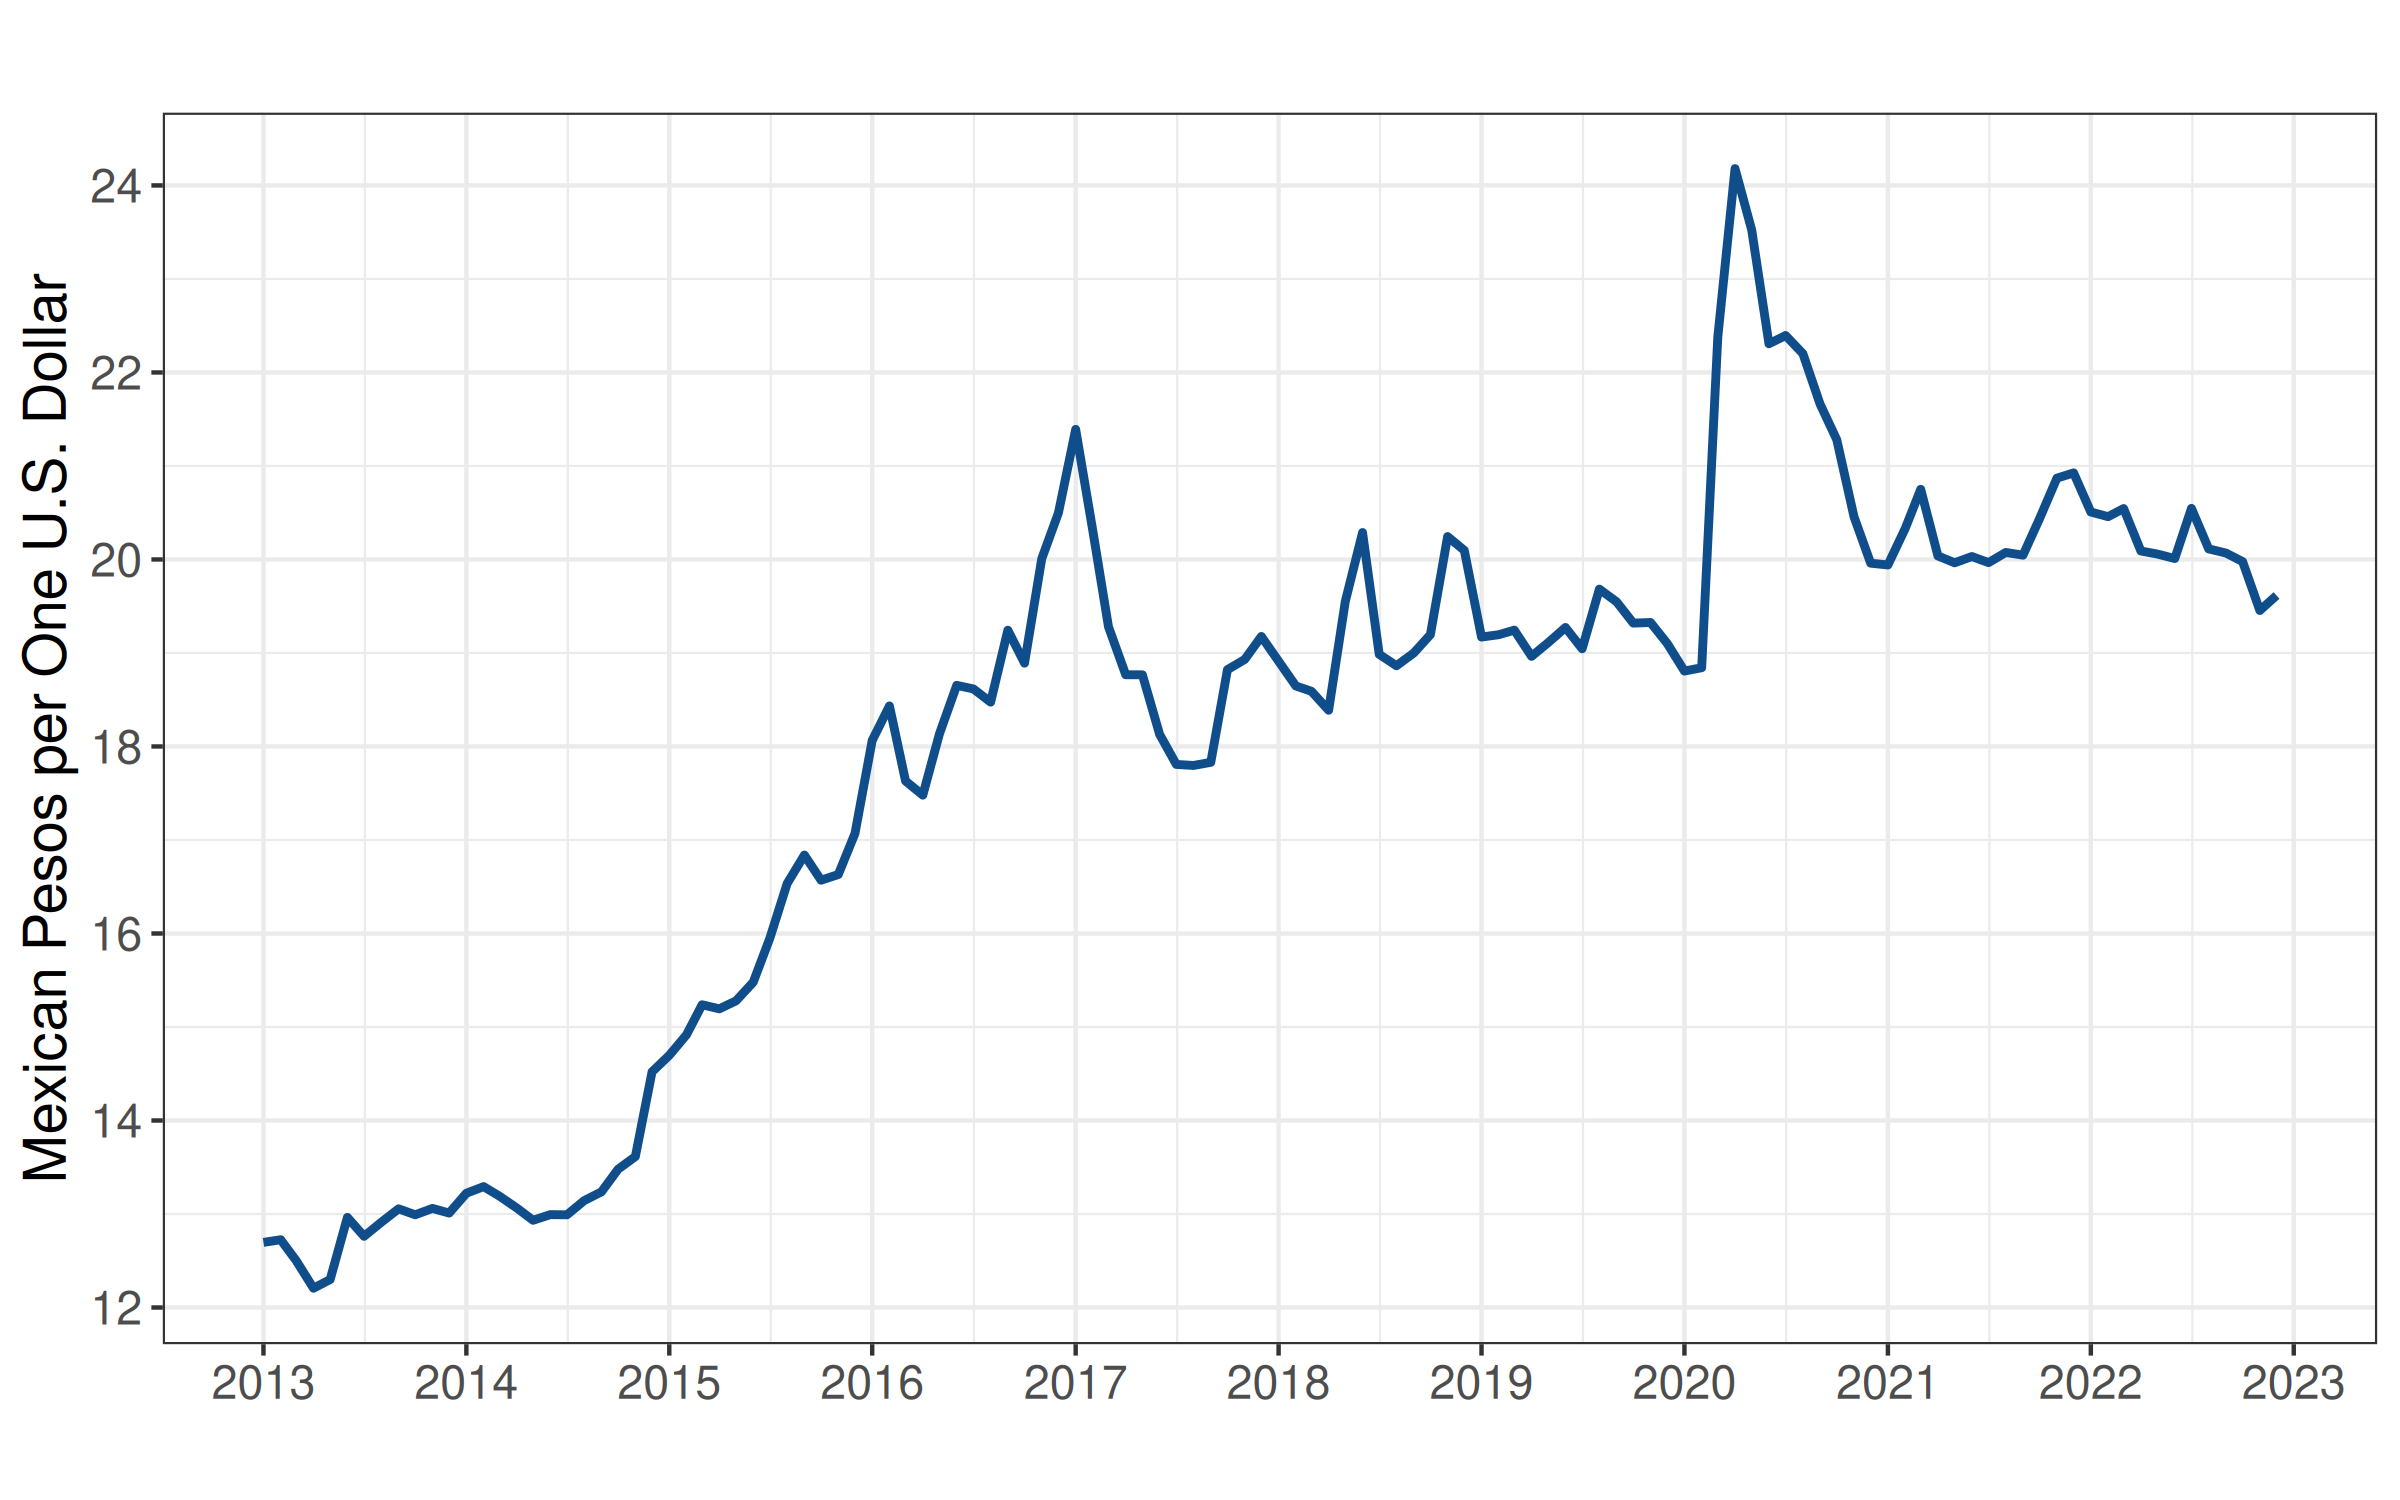
\includegraphics[width=\textwidth]{./R/mxn_usd.png}
\end{center}

\end{frame}

\begin{frame}
  \ft{Australia: U.S. Dollars per Australian Dollar}
  \begin{center}
  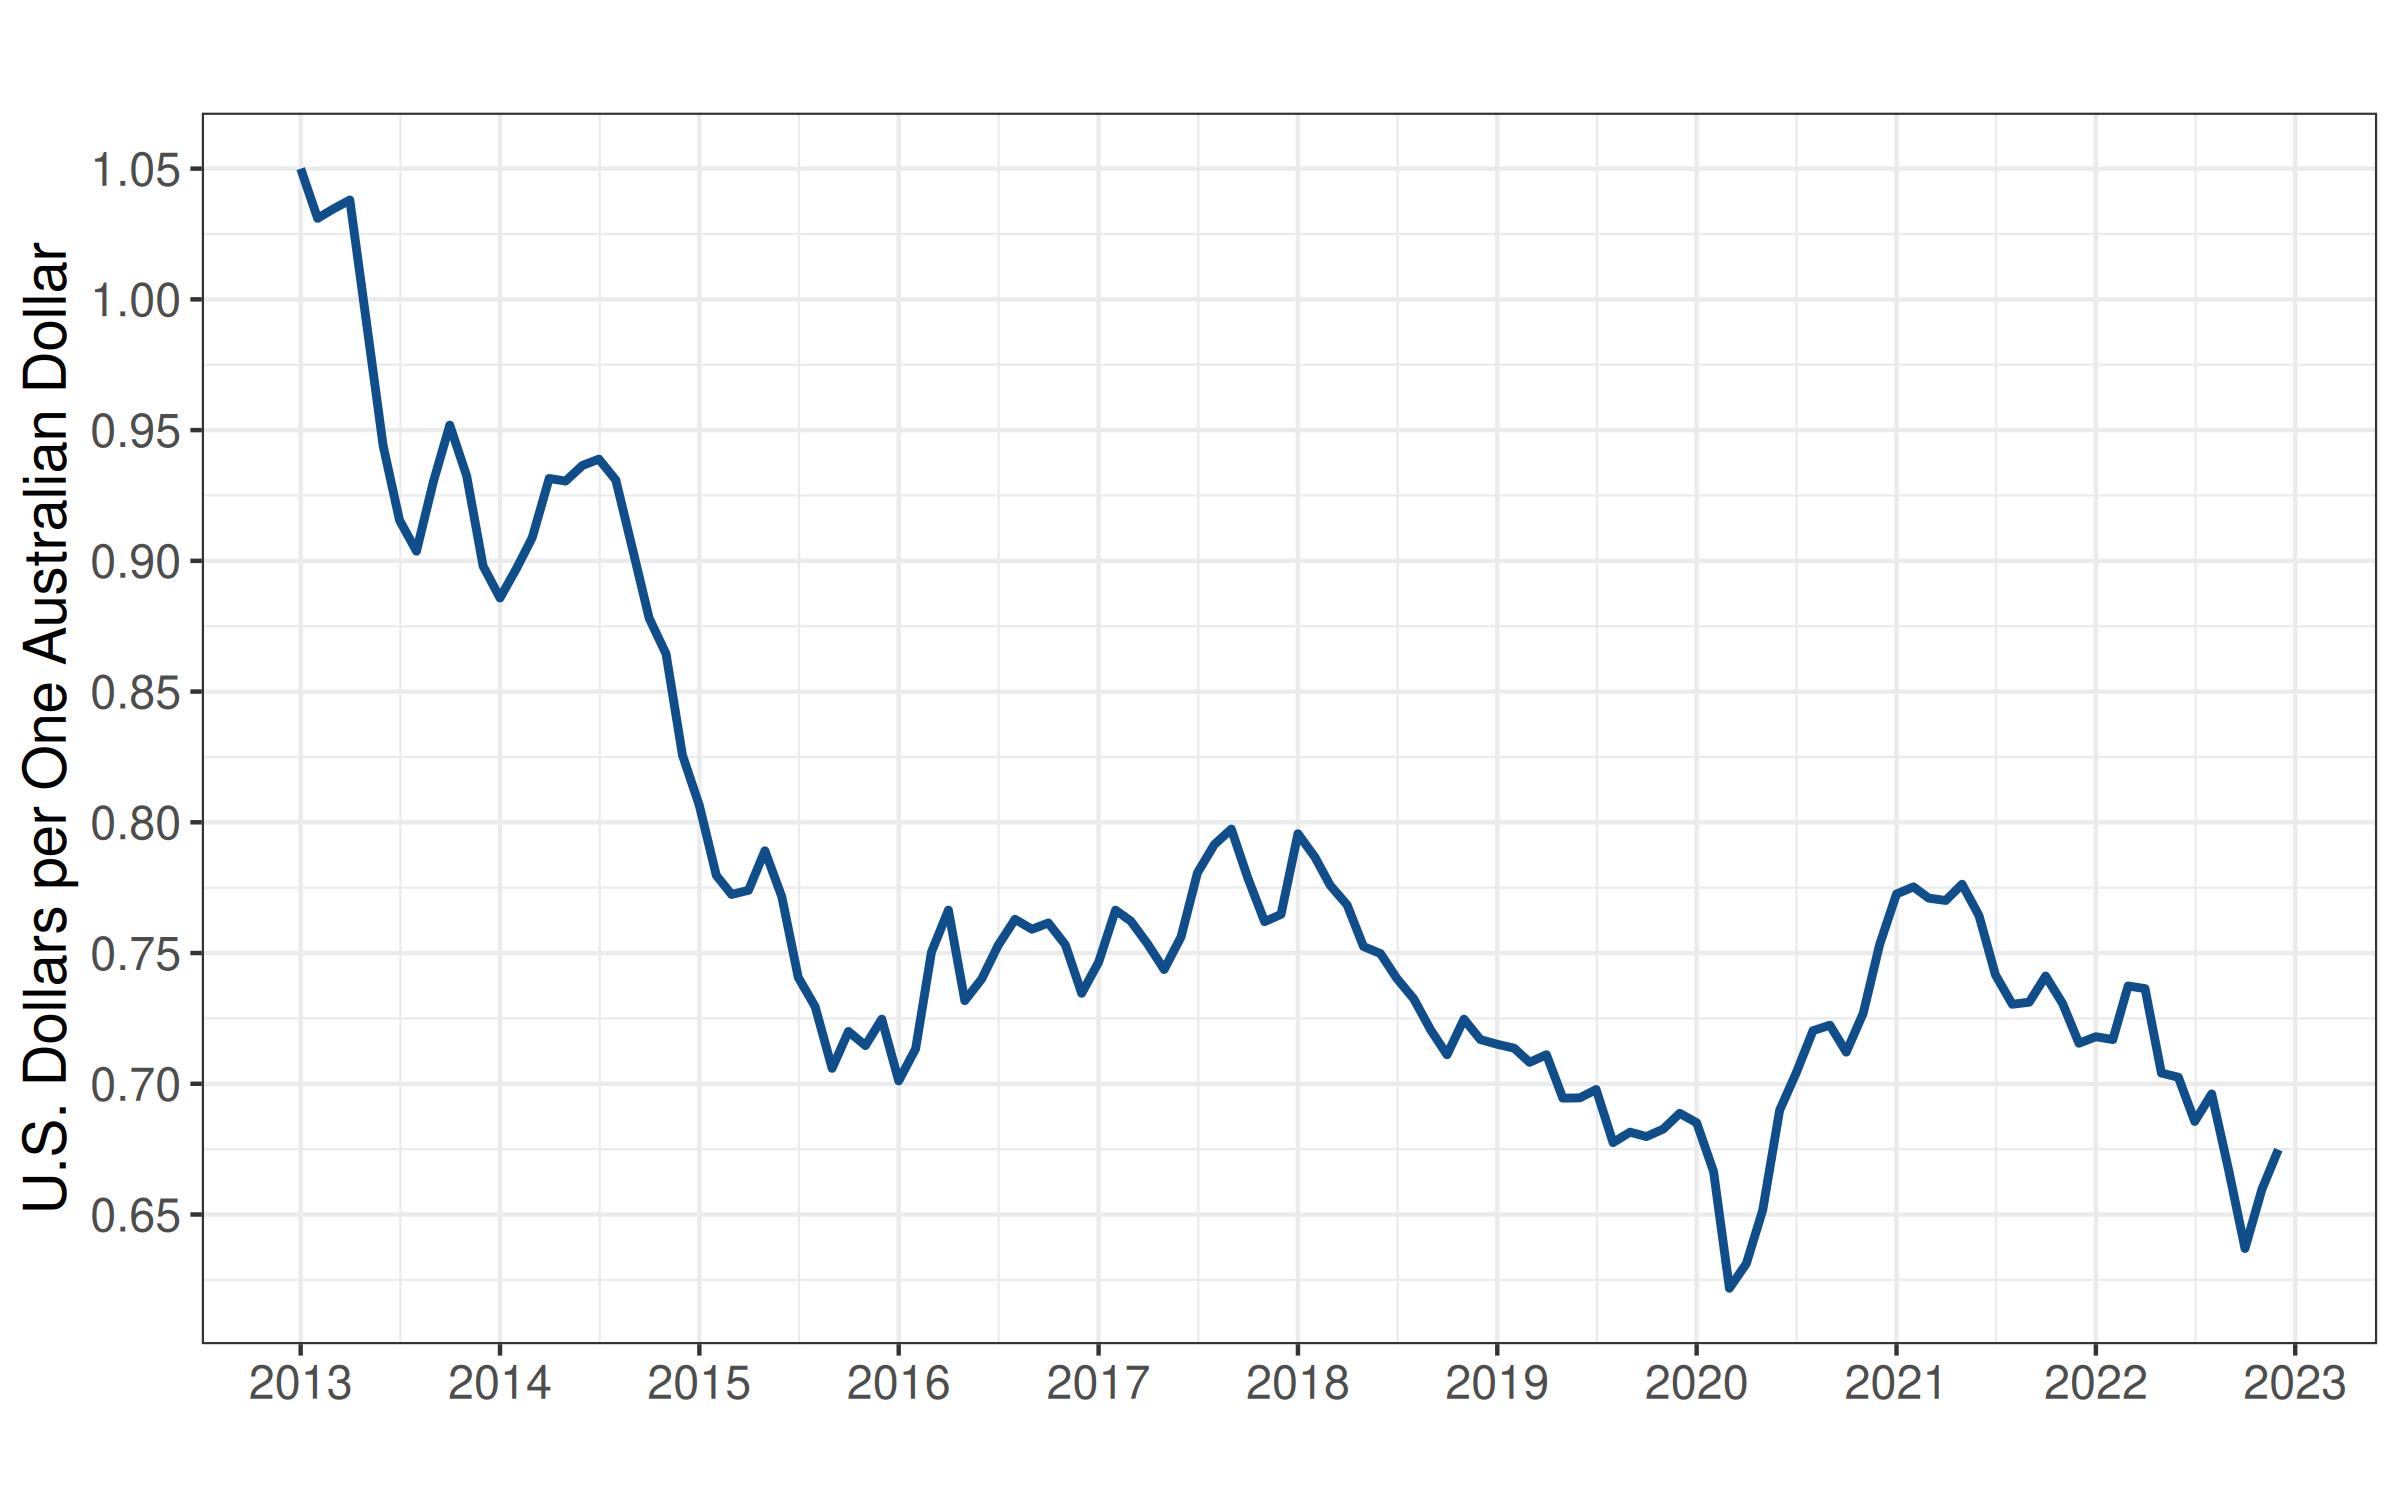
\includegraphics[width=\textwidth]{./R/aud_usd.png}
  \end{center}
\end{frame}

\begin{frame}
  \ft{Canada: Canadian Dollars per U.S. Dollar}
  \begin{center}
  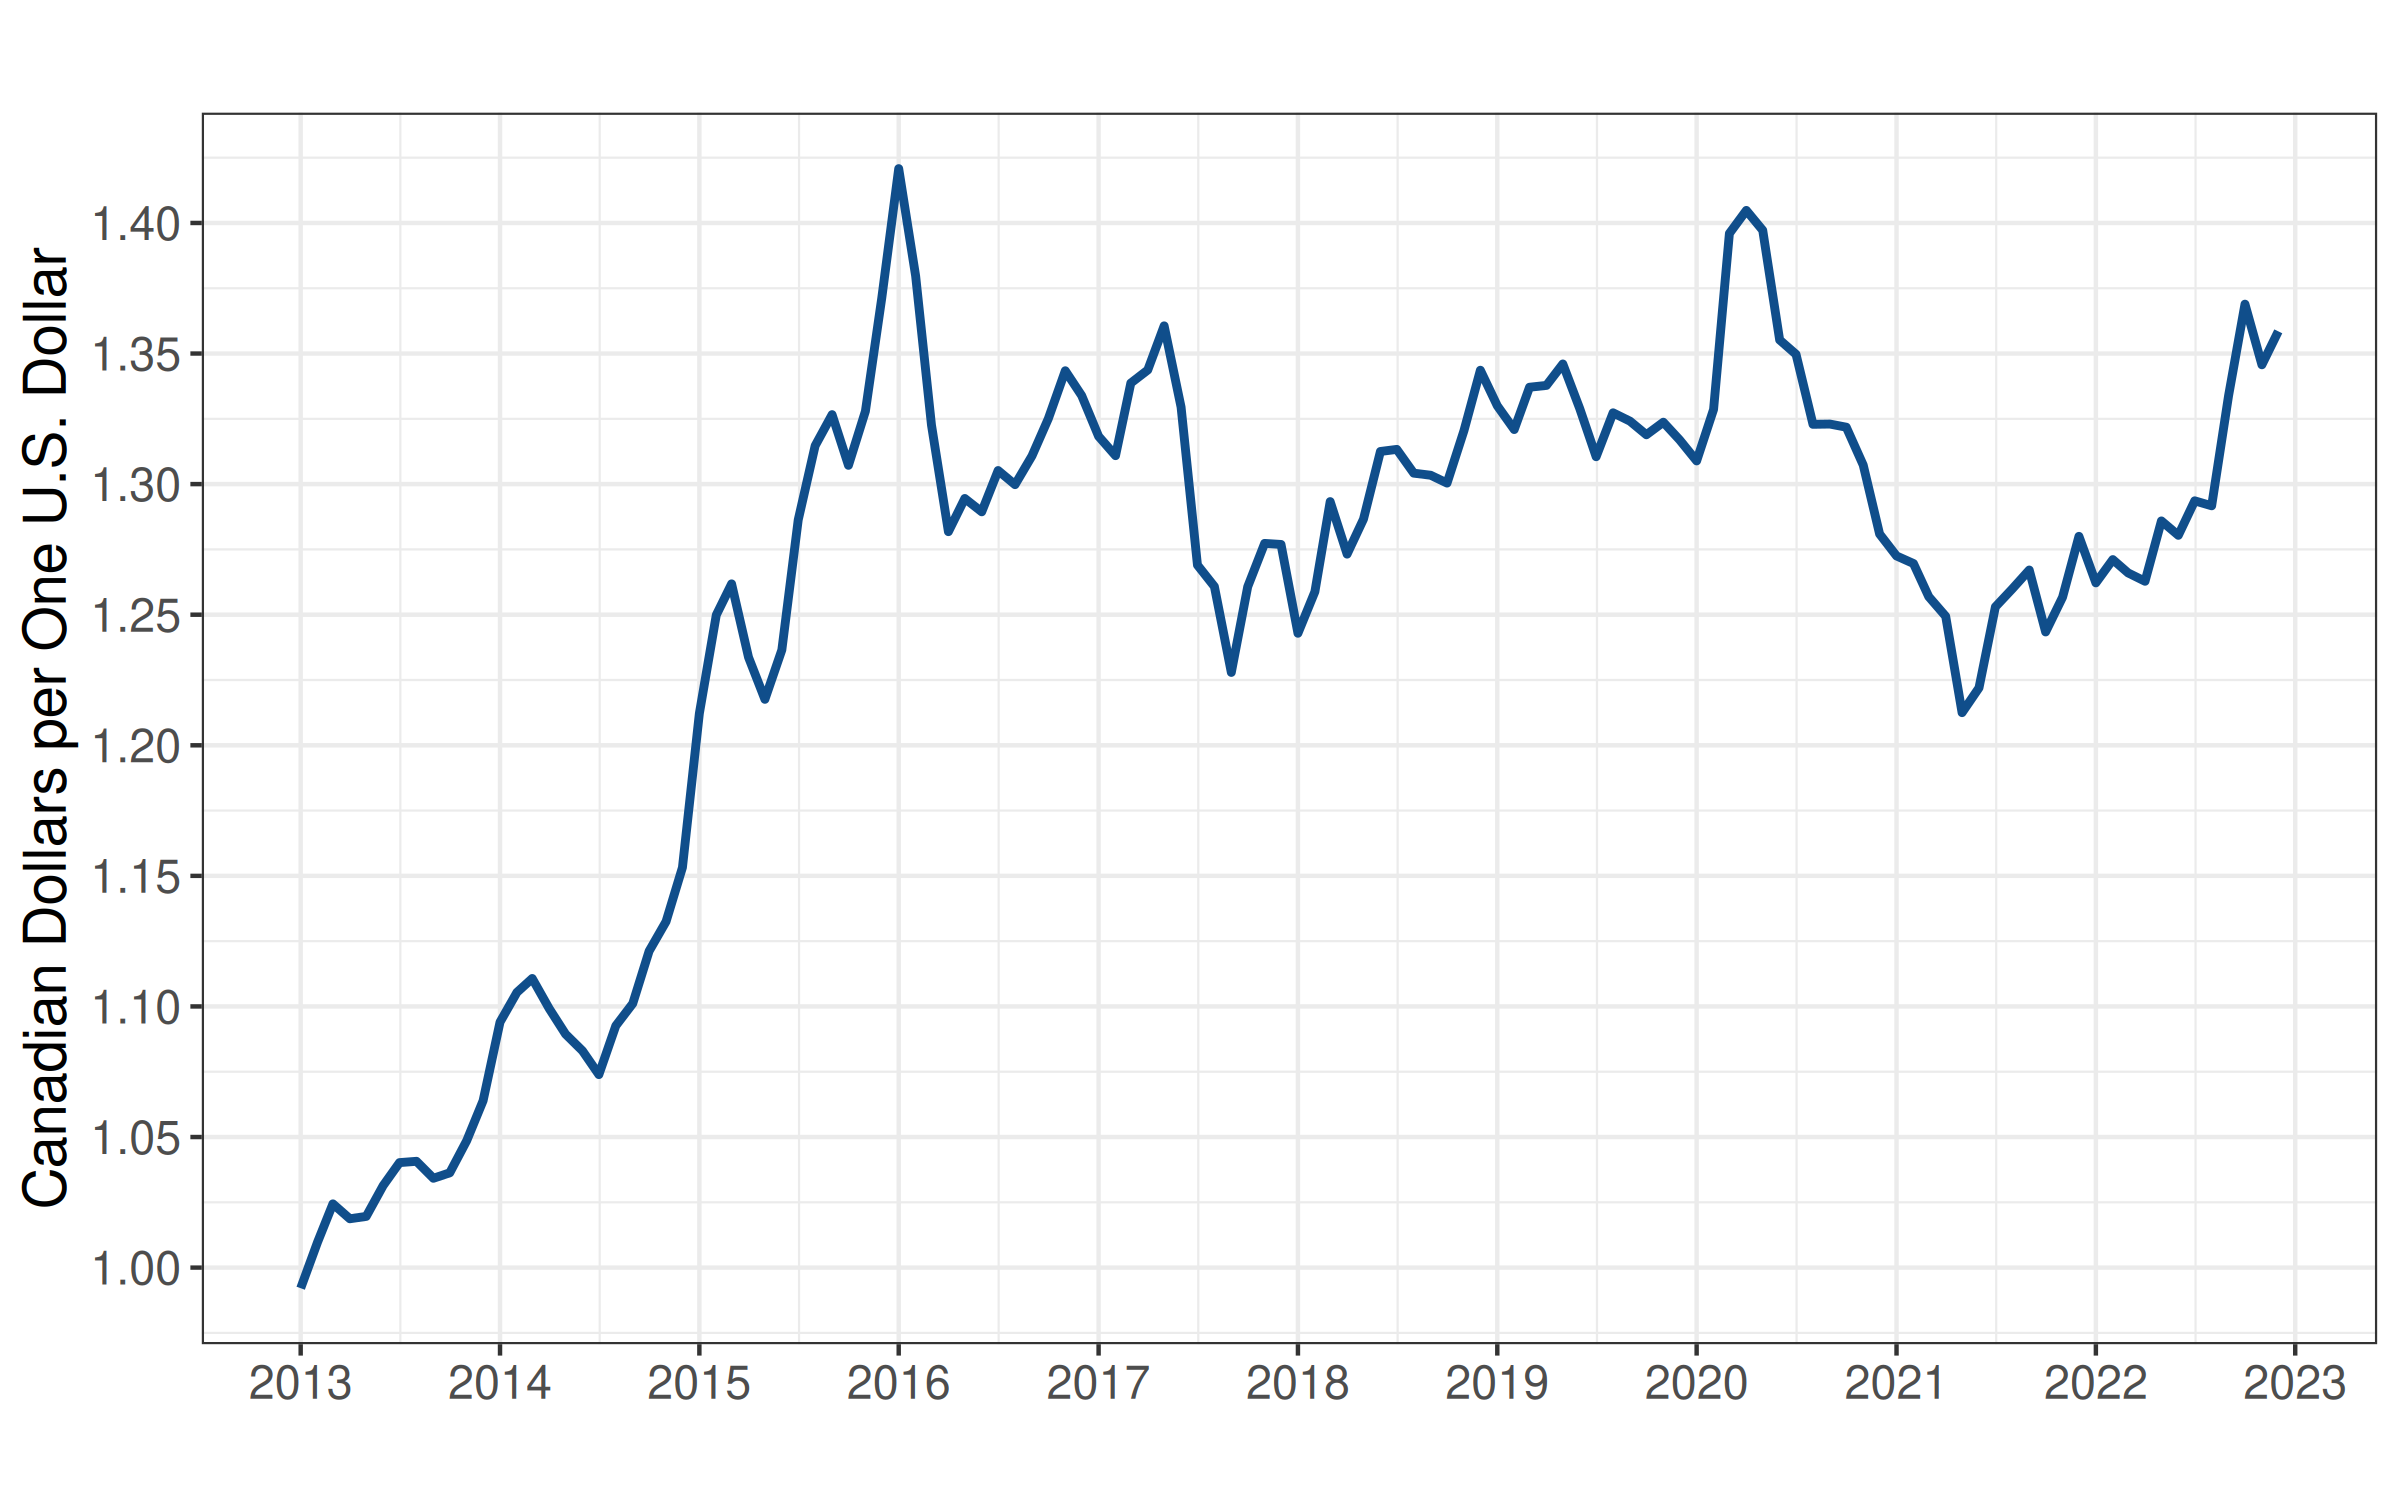
\includegraphics[width=\textwidth]{./R/cad_usd.png}
  \end{center}
\end{frame}


\begin{frame}
  \ft{China: Chinese Yuan per U.S. Dollar}
  \begin{center}
    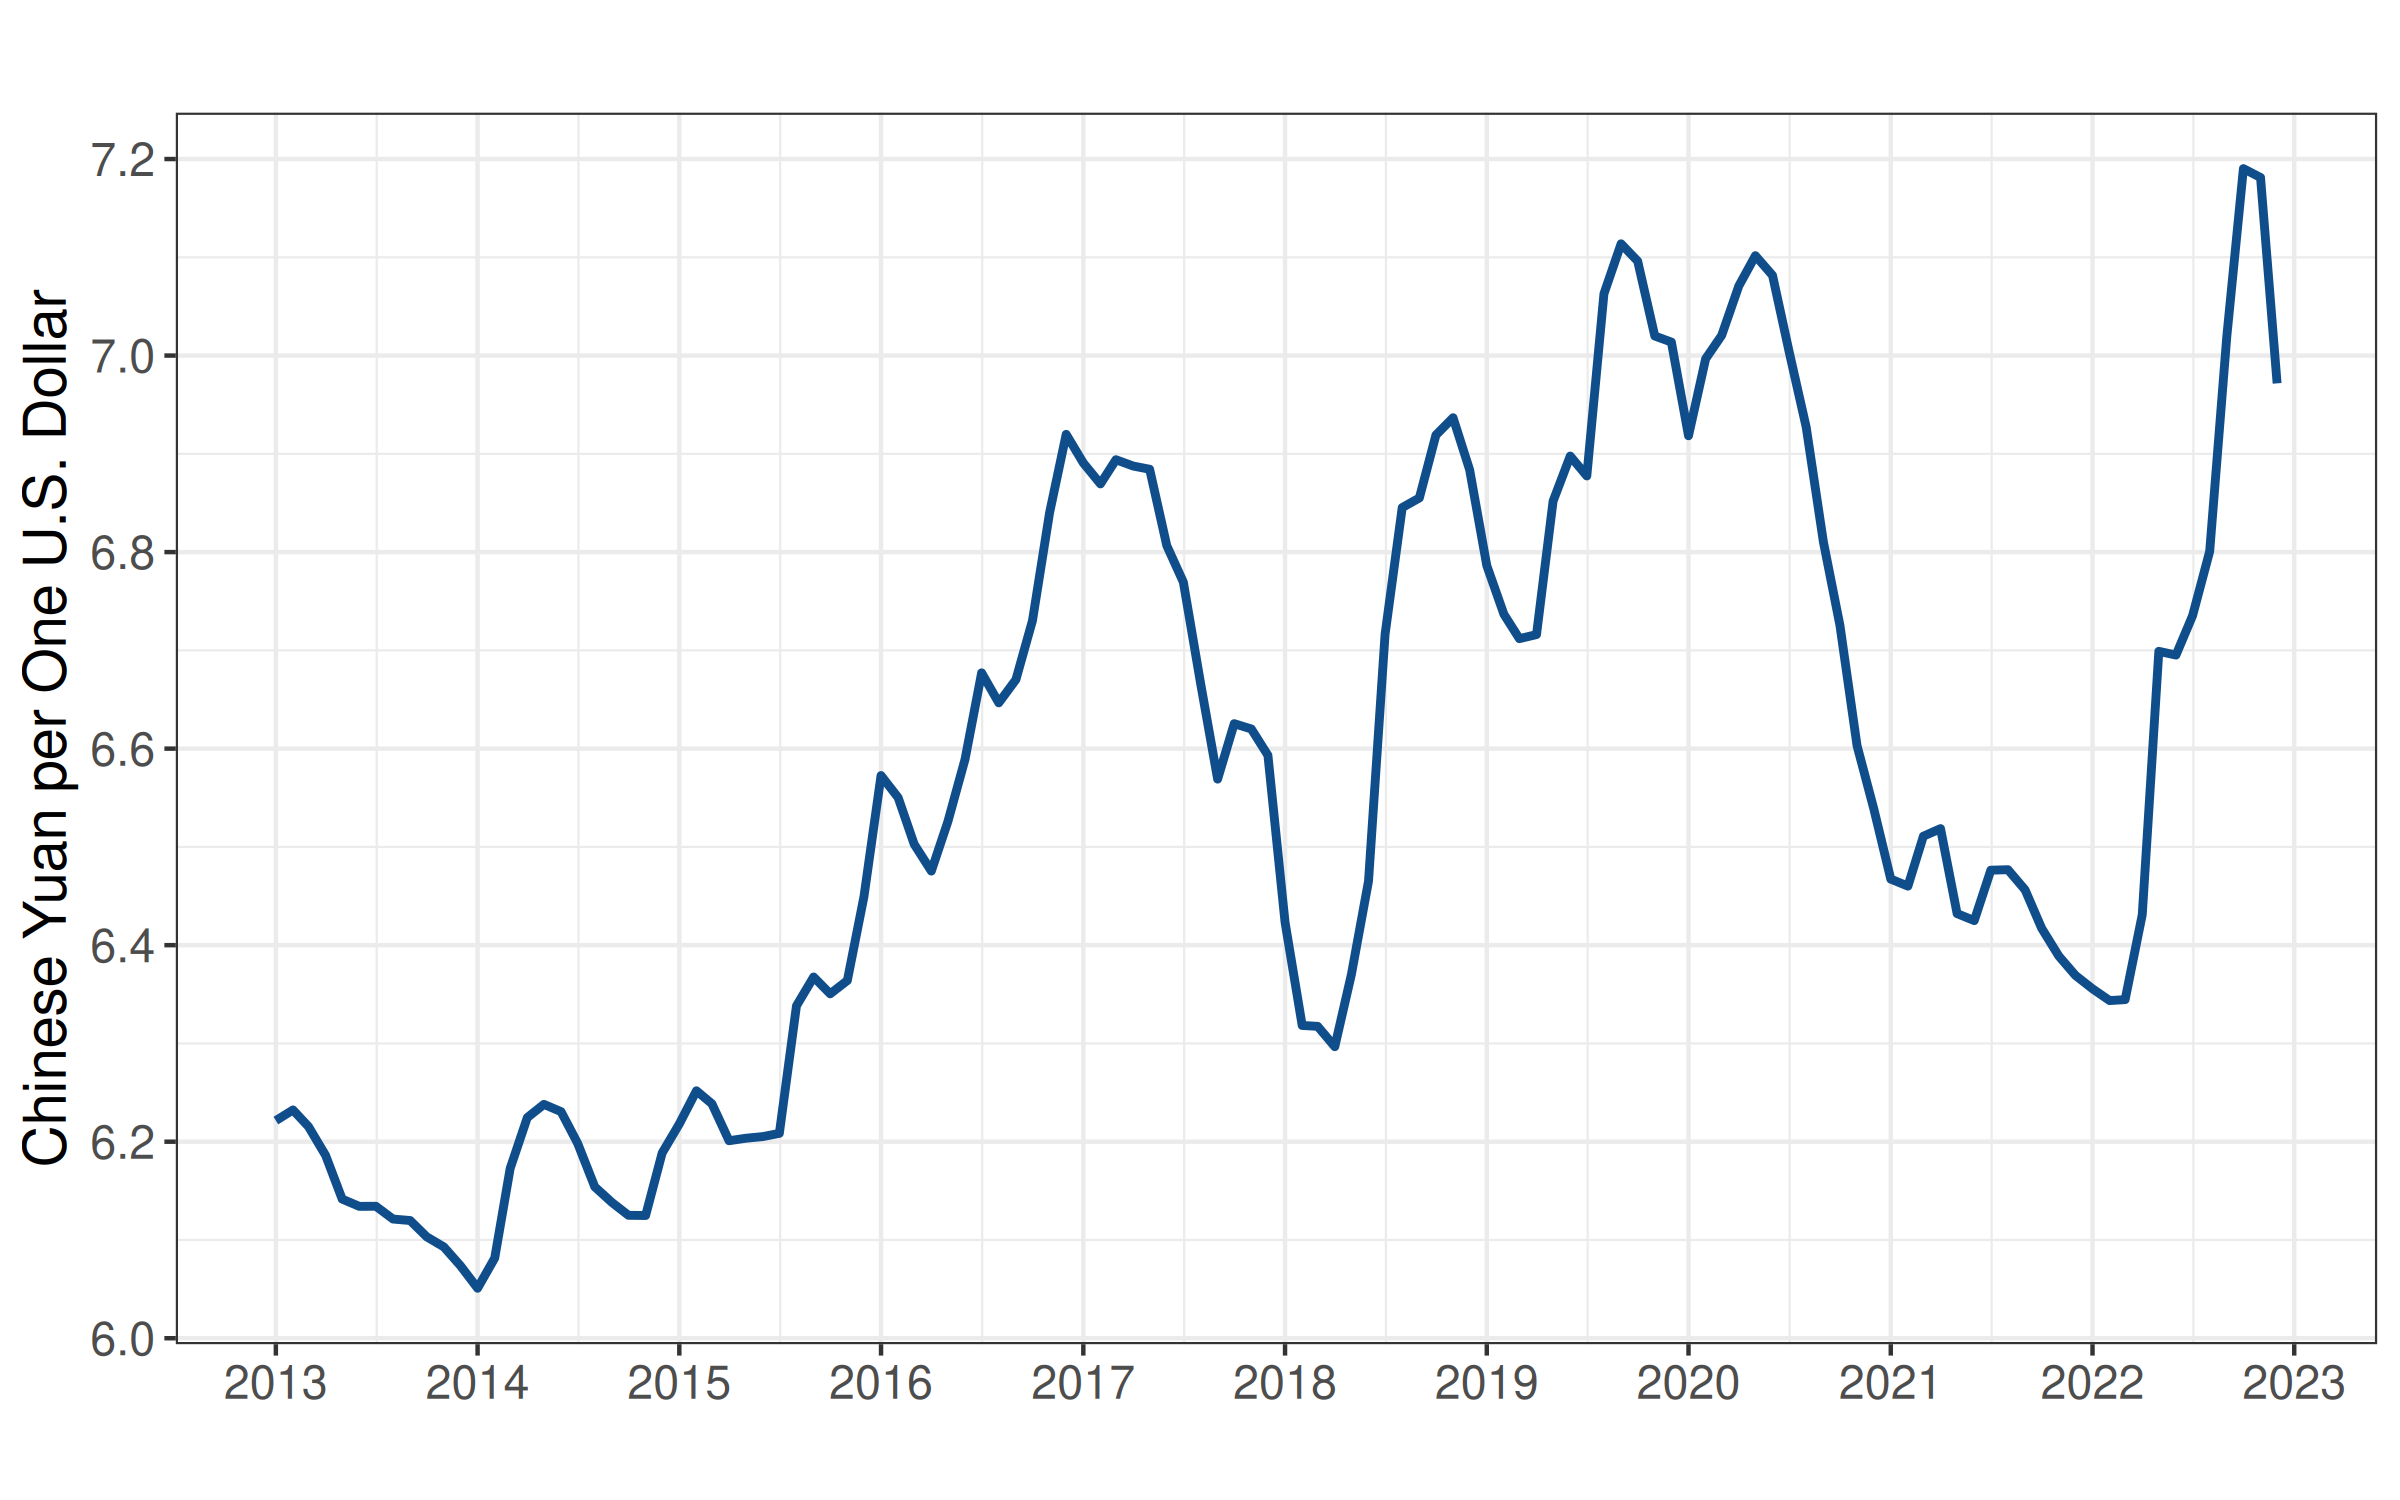
\includegraphics[width=\textwidth]{./R/cny_usd.png}
  \end{center}
\end{frame}


\begin{frame}
  \ft{Europe: U.S. Dollar per Euro}
  \begin{center}
    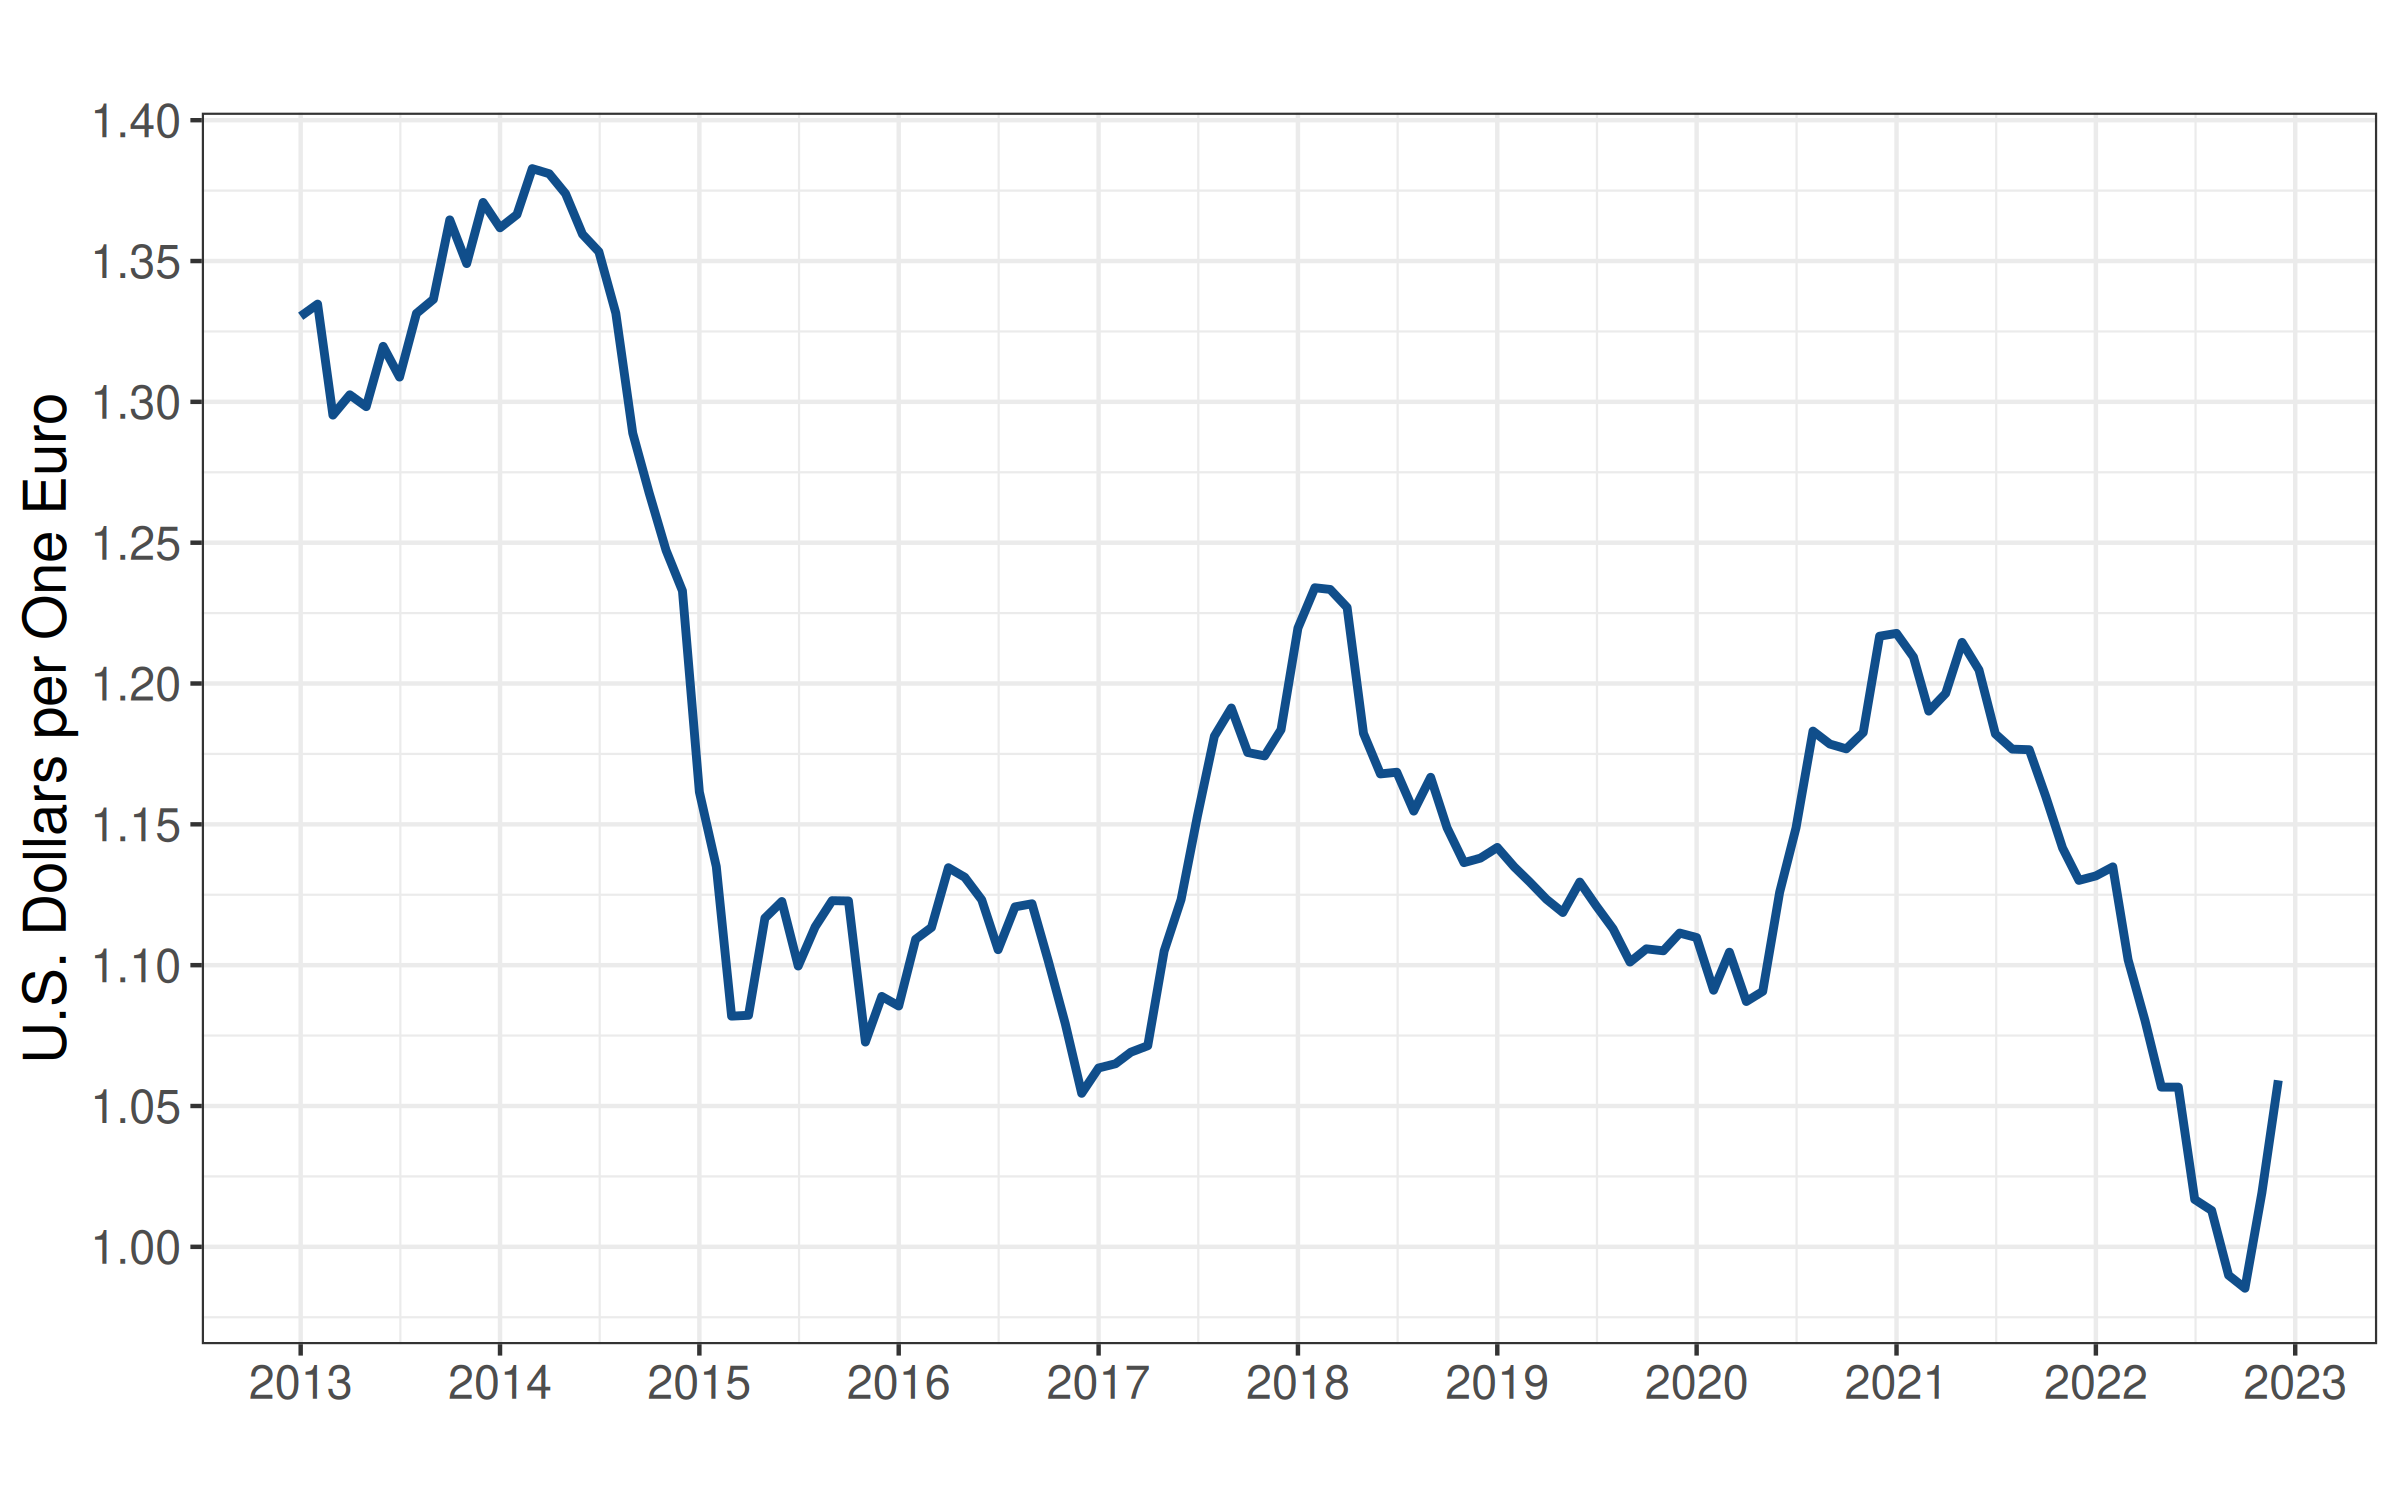
\includegraphics[width=\textwidth]{./R/eur_usd.png}
  \end{center}
\end{frame}


\begin{frame}
  \ft{Japan: Japanese Yen per U.S. Dollars}
  \begin{center}
    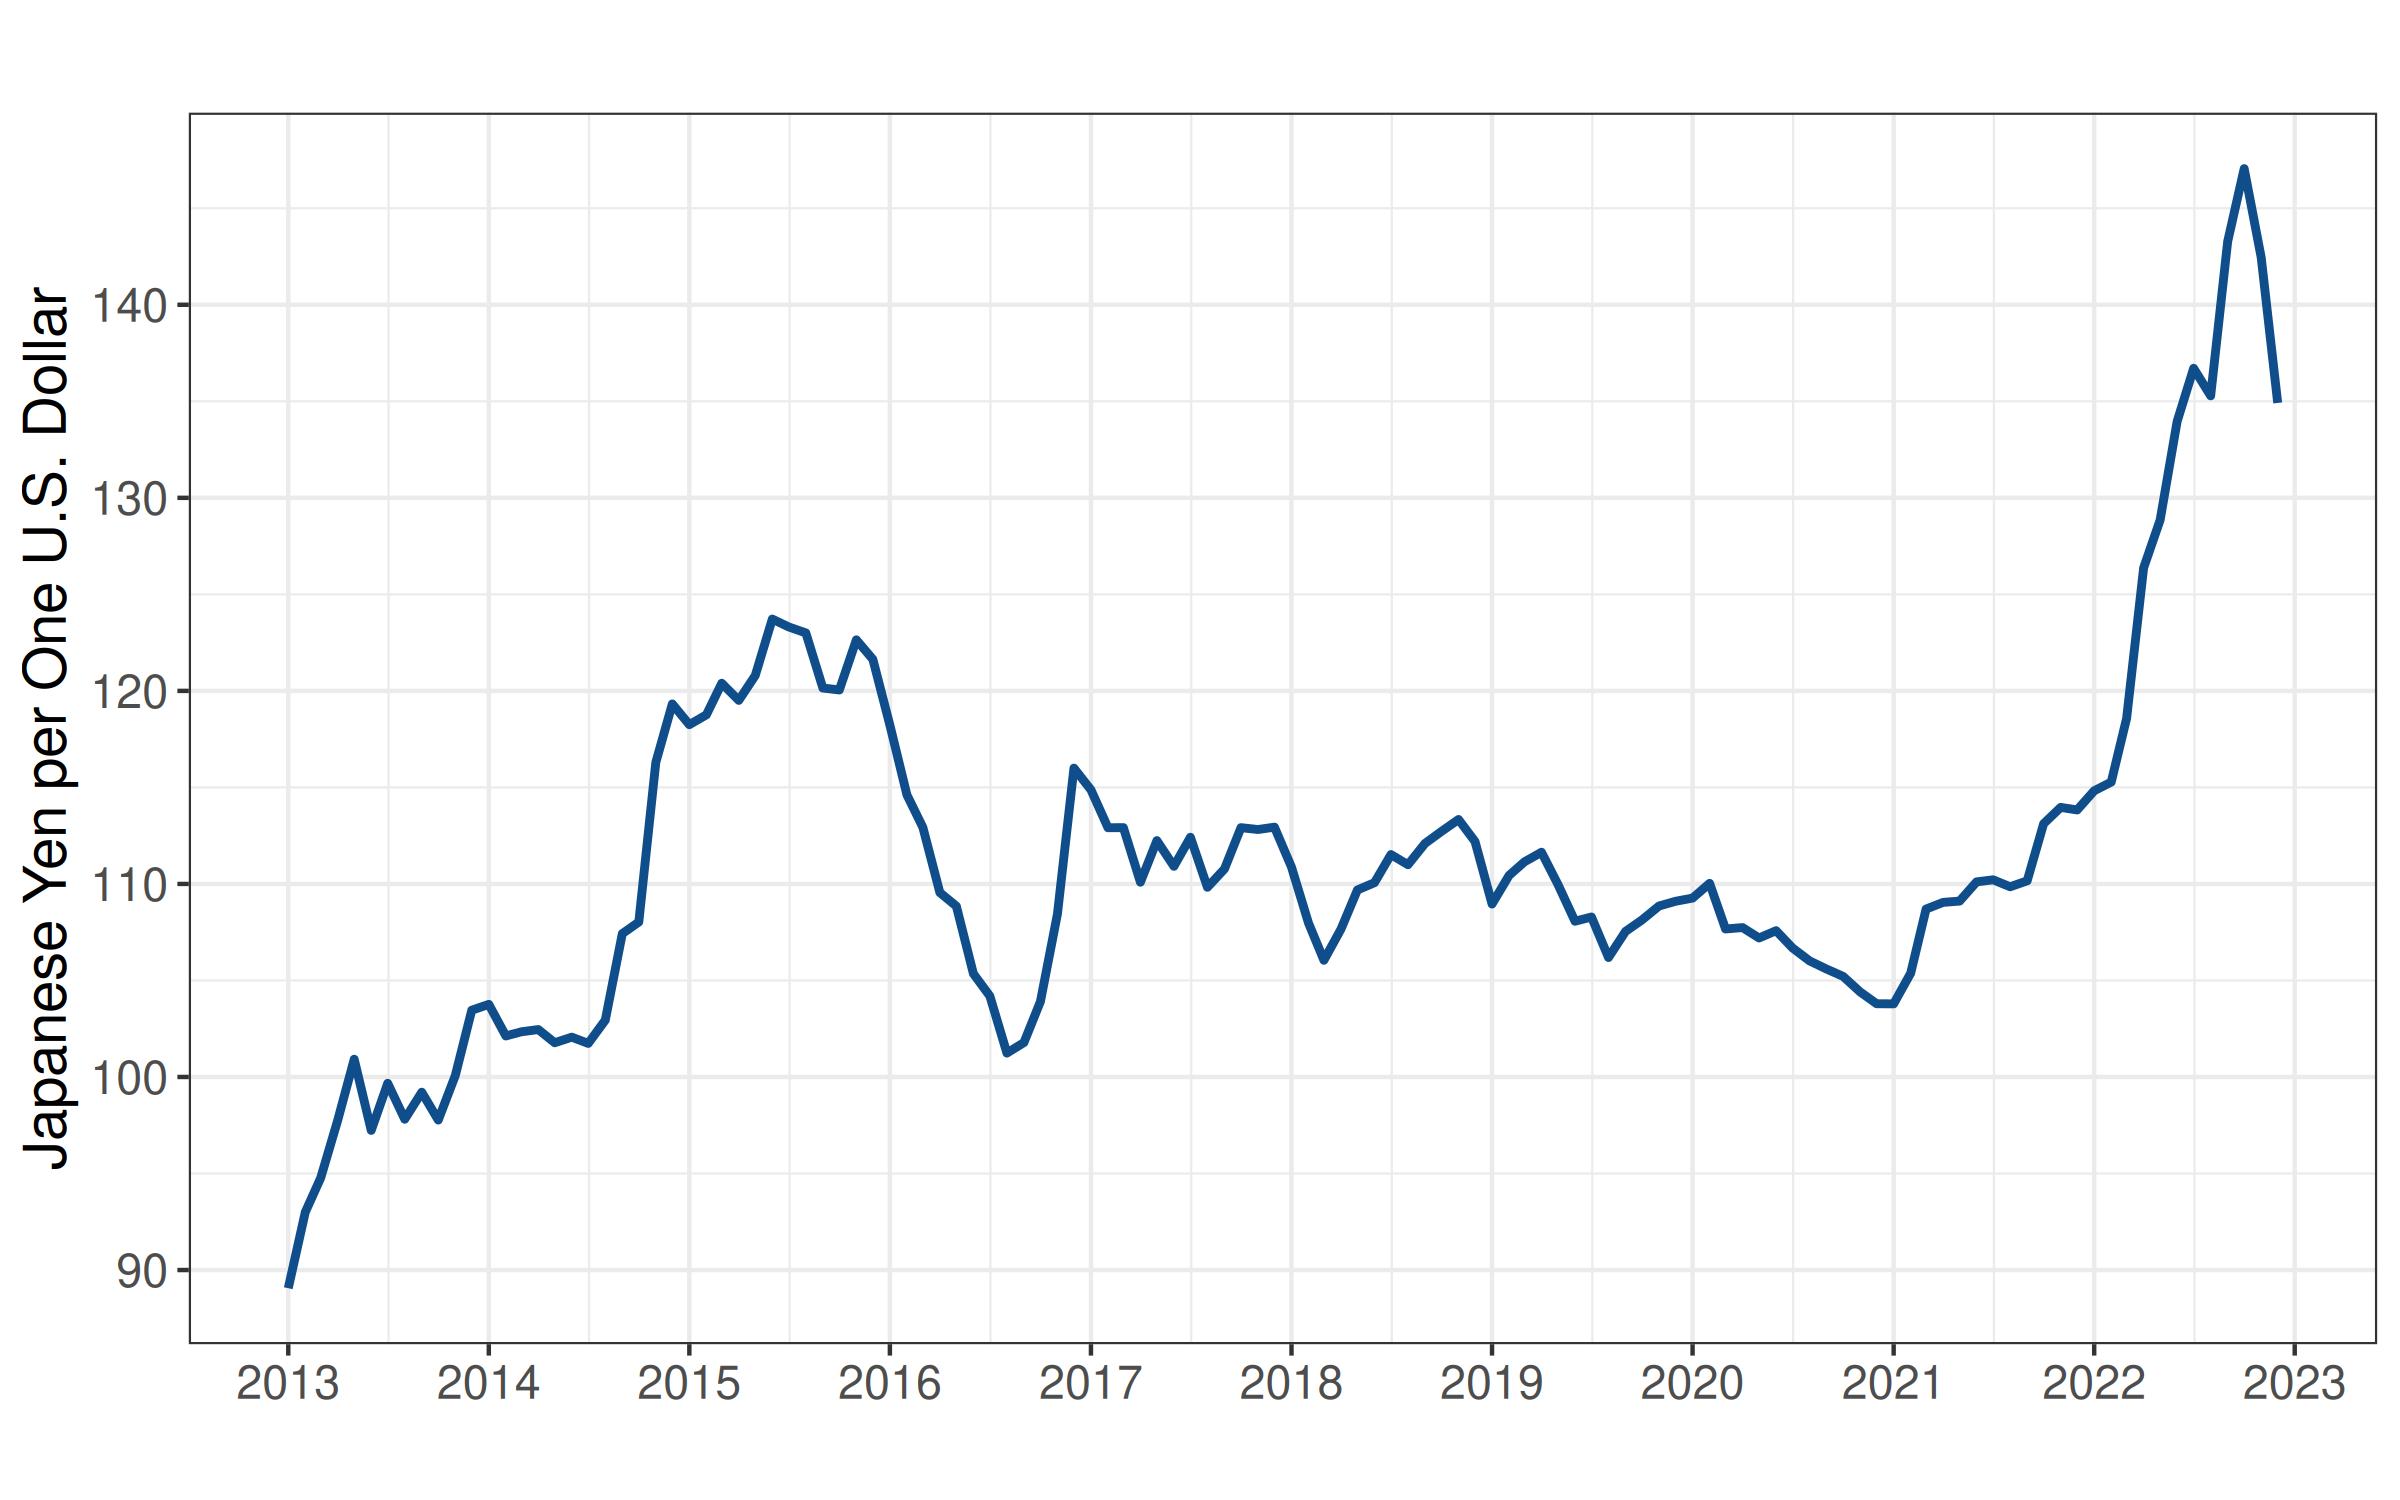
\includegraphics[width=\textwidth]{./R/jpy_usd.png}
  \end{center}
\end{frame}

\begin{frame}
  \ft{South Korea: Korean Won per U.S. Dollars}
  \begin{center}
    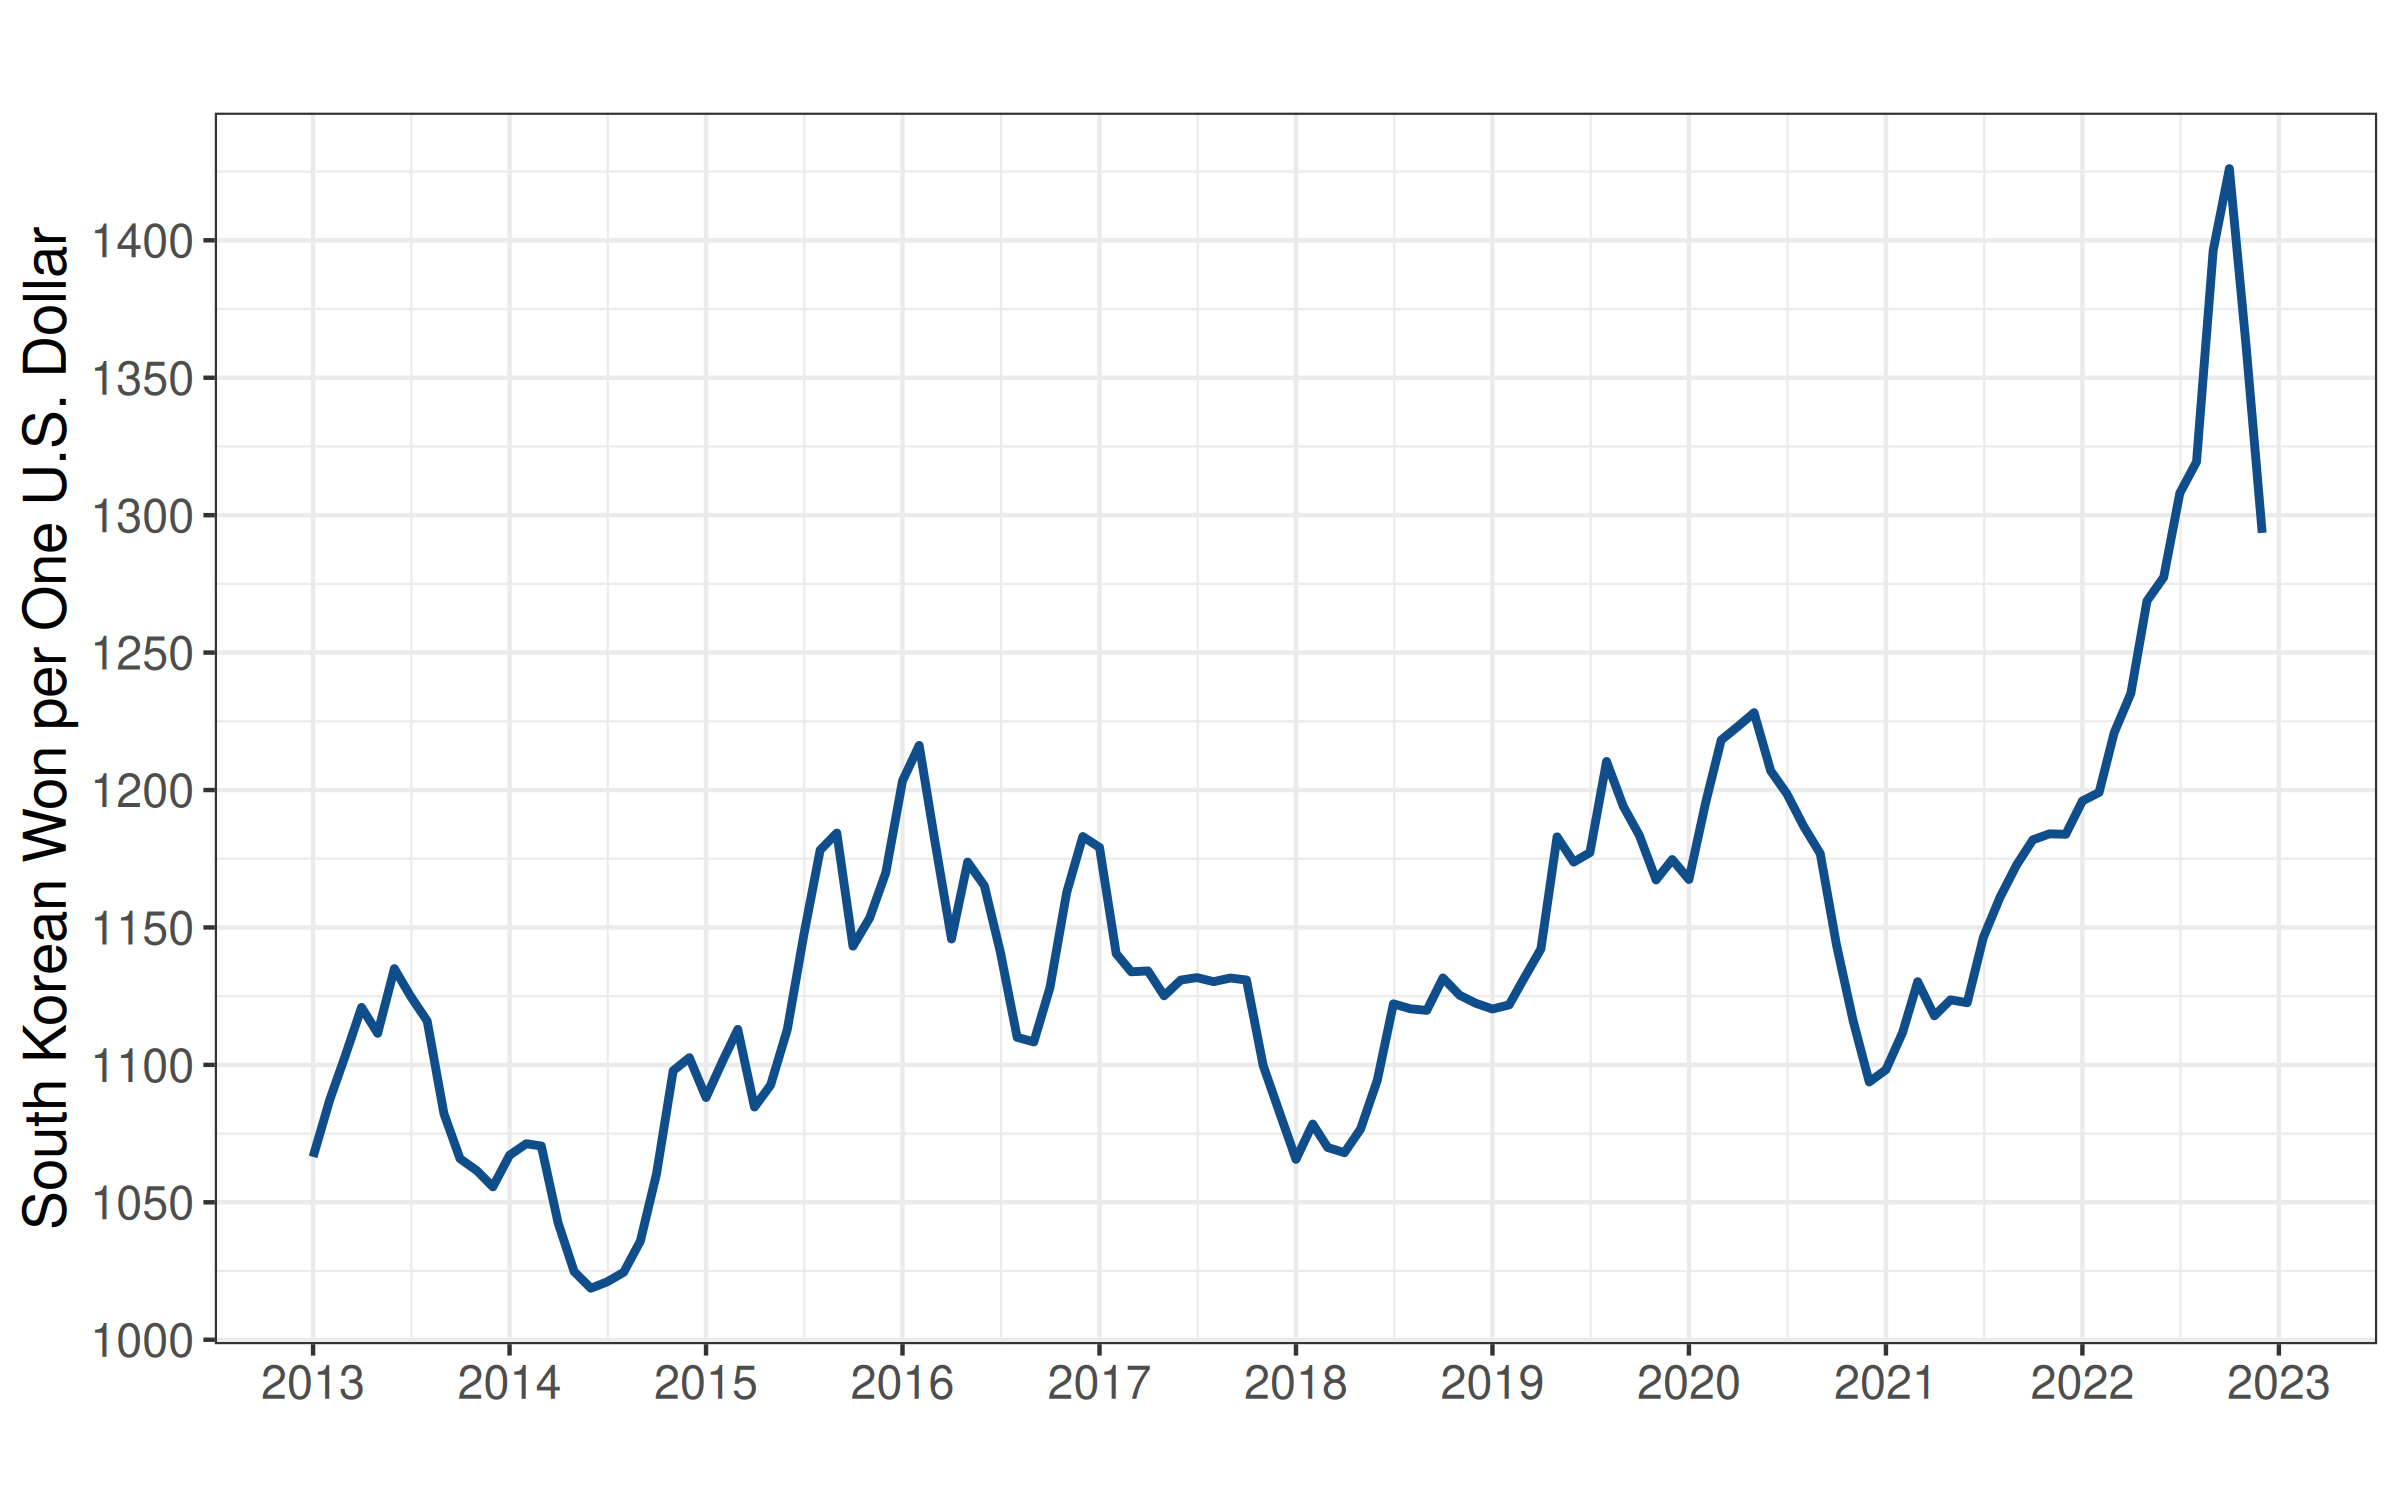
\includegraphics[width=\textwidth]{./R/krw_usd.png}
  \end{center}
\end{frame}

\begin{frame}
  \ft{Trade-Weighted Index}
  \begin{center}
    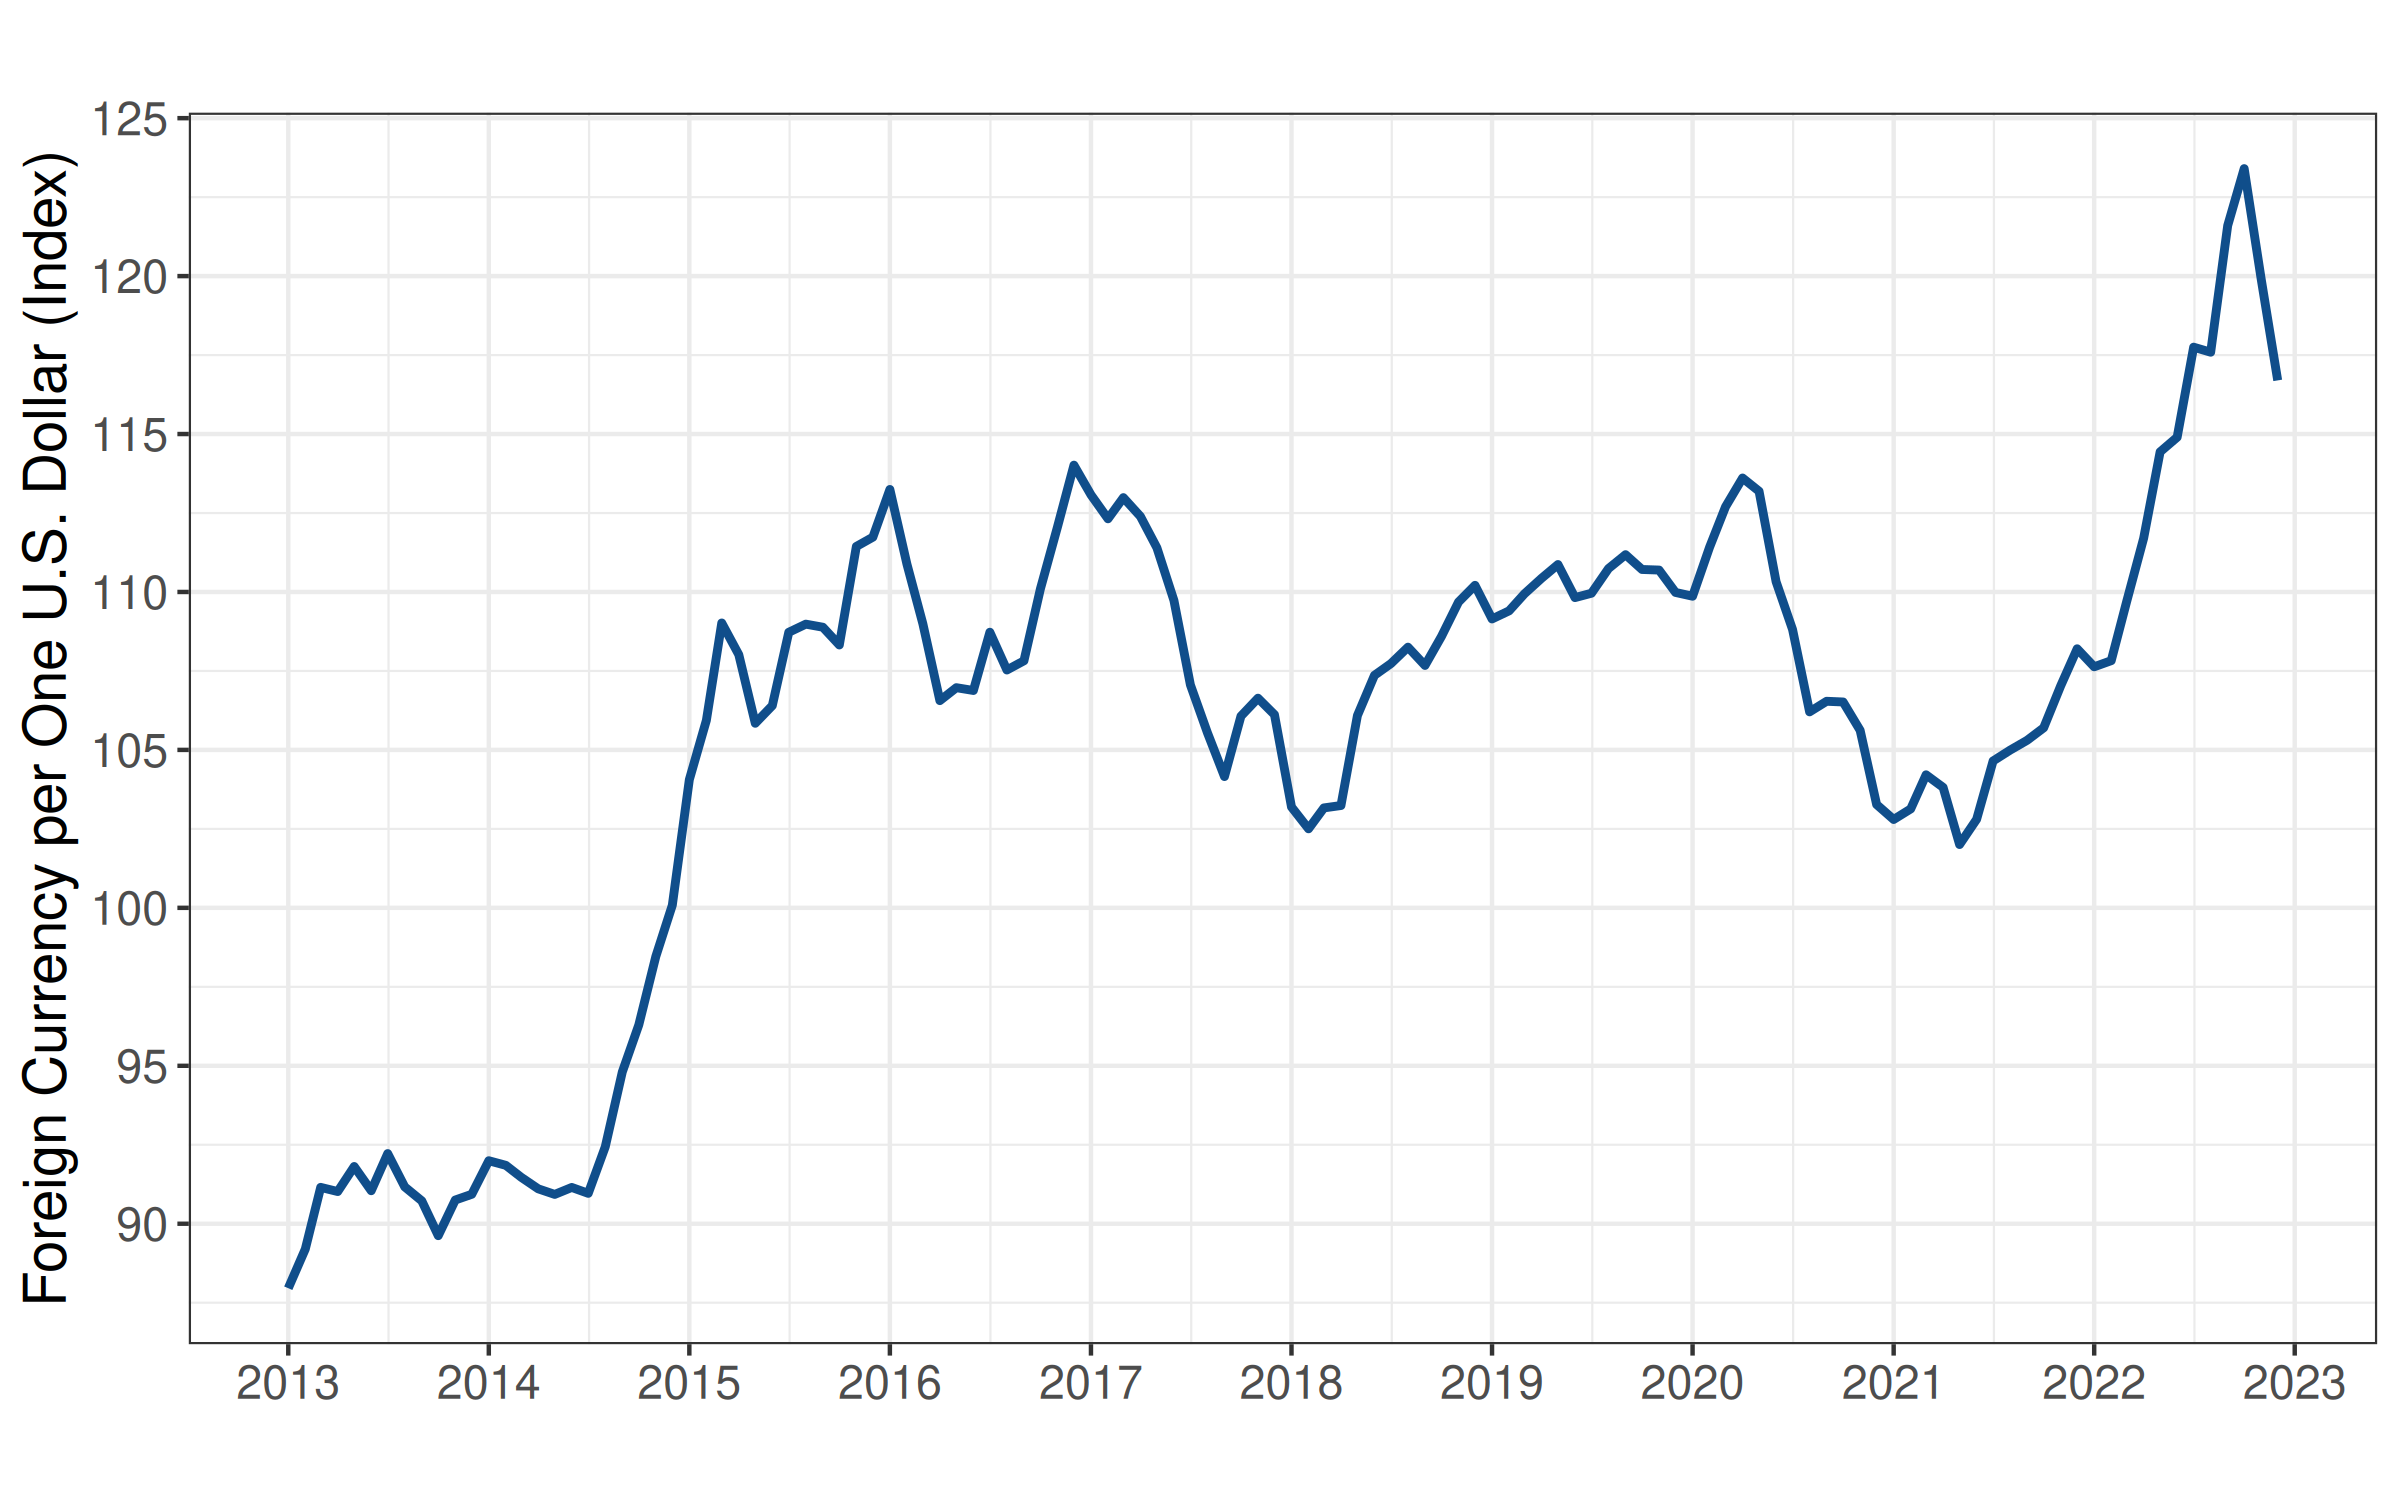
\includegraphics[width=\textwidth]{./R/trade.png}
  \end{center}

  \vspace*{-0.25in}
  \begin{scriptsize}
    \begin{itemize}
      \item Weighted average of many currencies, based on level of trade.
      \item Includes: Euro Area, Canada, Japan, United Kingdom, Switzerland, Australia, and Sweden.
    \end{itemize}
  \end{scriptsize}
\end{frame}

\section{Supply and Demand}
\subsection{Demand for Currency}
\frame
{
  \ft{Demand for Currency}
  \bi
  \item<+-> Price of currency of interest (say U.S. Dollars):
    \bi
    \item<+-> Exchange rate expressed as foreign currency per one unit of currency of interest.
    \item<+-> Example: price of dollars = Euros per U.S. dollar.
    \item<+-> An increase in this exchange rate means an appreciation of the dollar.
    \ei
  \item<+-> Demand for currency is a \textit{derived demand}.  It depends on...
    \bi
    \item<+-> \textit{foreign demand} for the country's goods.
    \item<+-> \textit{foreign demand} for the country's assets.
    \item<+-> Financial assets could include stocks and bonds for companies in a country, government bonds from a country
    \item<+-> Assets may include foreign direct investment, when owners from a foreign country own significant portions of a company or a company's facilities located in a country.
    \ei
  \ei
}

\frame
{
  \ft{Demand for Currency}
  \bi
  \item<+-> \textbf{Law of demand for foreign exchange:} as the value of the currency increases, the quantity of the currency demanded will fall.
  \item<+-> \textbf{Exports effect:} if the currency is more expensive, the country's goods are more expensive.
  \ei
}

\frame
{
  \ft{Shifts in Demand}
  \bi
  \item<+-> When something \textit{besides the exchange rate} influences the demand for a currency, then there is a \textit{shift} in the demand.
  \item<+-> Determinants of demand for currency:
    \bi
    \item<+-> Changes in demand for country's products.
    \item<+-> Changes in interest rate differential.
    \item<+-> Expectations of future exchange rate.
    \ei
  \ei
}

\subsection{Supply of Currency}
\frame
{
  \ft{Supply of Currency}
  \bi
  \item<+-> A currency is supplied when holders of the currency try to sell it.
  \item<+-> Supply of U.S. dollars happens when people in U.S. demand foreign currencies.
  \item<+-> Supply of a currency is nothing more than the holders' demands for foreign currency.
  \ei
}

\subsection{Examples}
\frame
{
  \ft{Example 1: Decrease in Income in Korea}
  \scriptsize{
  Japan and Korea are major trading partners. Suppose there is a decrease in incomes in Korea, leading to a decrease in demand for imported goods from Japan to Korea
  \begin{center}
    \only<1>{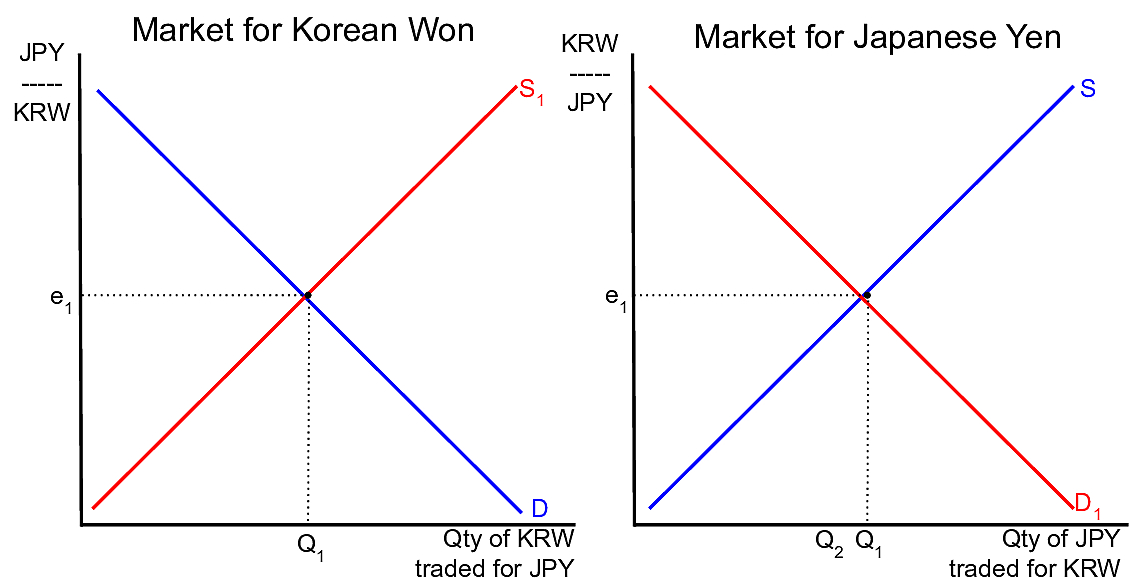
\includegraphics[width=0.8\linewidth]{./images/exchangerates-decreasedemand-JPY-KRW-start.jpg}}
    \only<2->{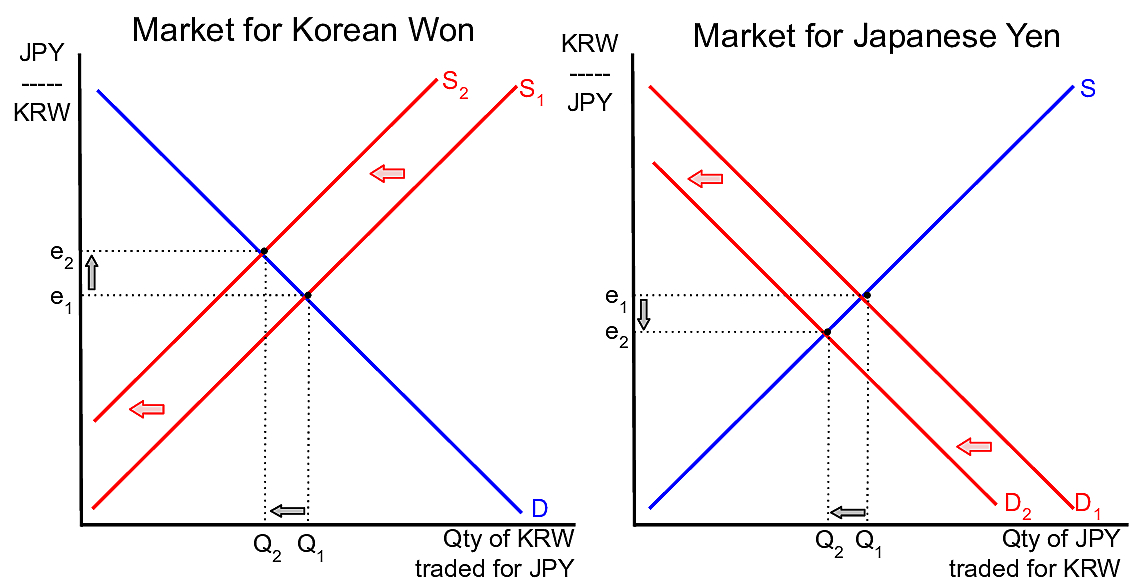
\includegraphics[width=0.8\linewidth]{./images/exchangerates-decreasedemand-JPY-KRW.jpg}}
  \end{center}
  \only<1>{Two related markets.  Market for Korean Won (Price=JPY/KRW)\newline and Market for Japanese Yen (Price=KRW/JPY)}
  \only<2>{Decrease in Koreans' demand for Japanese Yen\newline$\rightarrow$ Decrease in Supply of Korean Won.}
  \only<3>{Korean Won appreciates against the Japanese Yen \newline Equivalently, Japanese Yen depreciates against Korean Won}
}}


\frame
{
  \ft{Example: Reduction in Trade Restrictions}
  \begin{scriptsize}
  Suppose a trade agreement between Mexico and Canada results in a significant reduction in legal restrictions in Mexico, allowing more imports from Canada.
  \begin{center}
    \only<1>{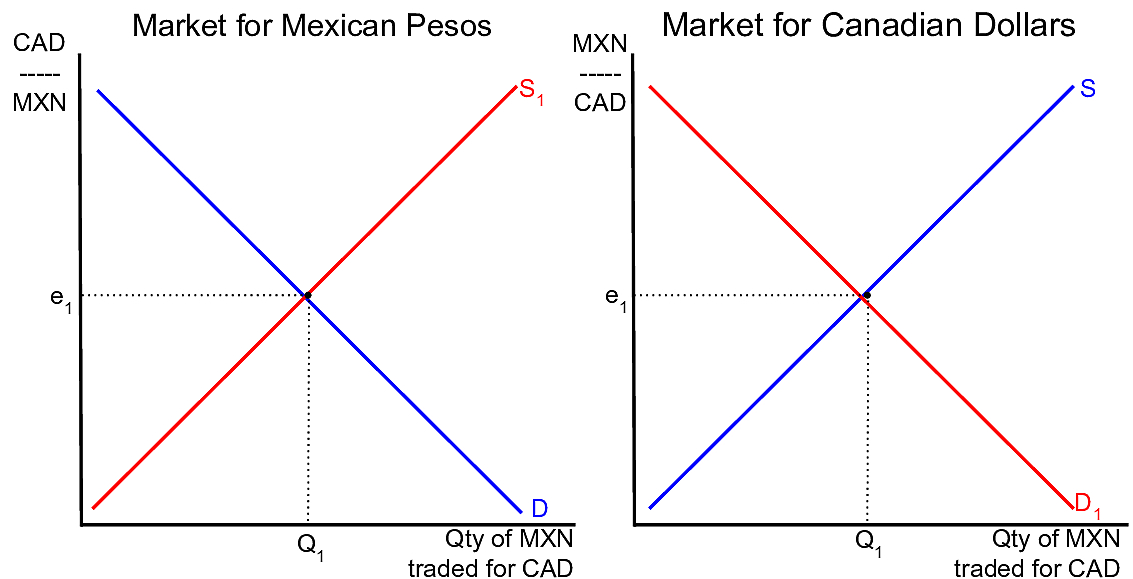
\includegraphics[width=0.8\linewidth]{./images/exchangerates-increasedemand-CAD-MXN-start.jpg}}
    \only<2->{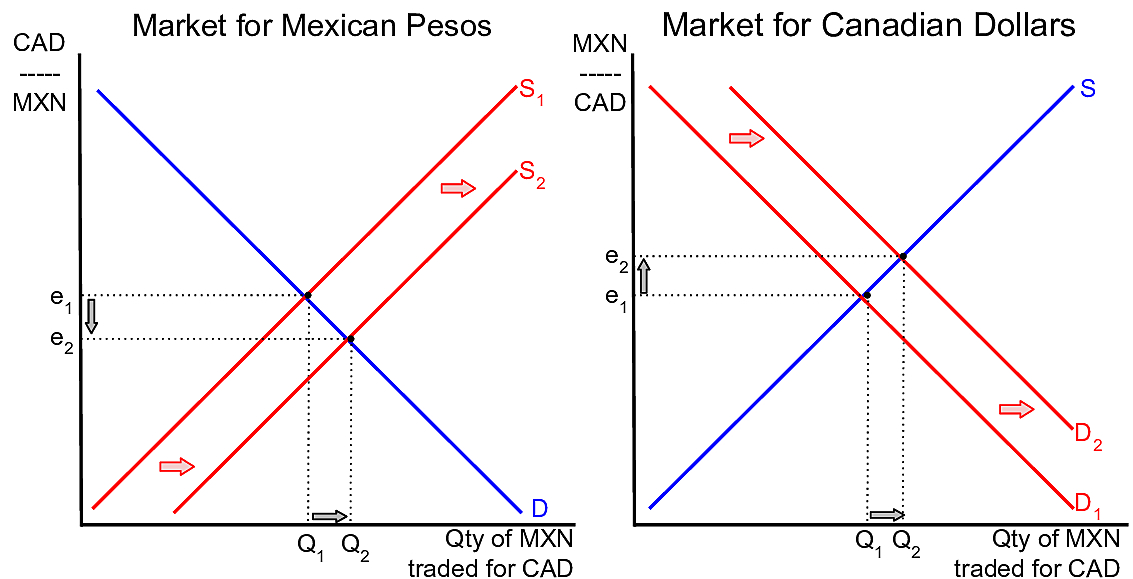
\includegraphics[width=0.8\linewidth]{./images/exchangerates-increasedemand-CAD-MXN.jpg}}
  \end{center}
  \only<1>{Two related markets.  Market for Mexican Pesos (Price=CAD/MXN)\newline and Market for Canadian Dollars (Price=MXN/CAD)}
  \only<2>{Increase in Mexican consumers' demand for Canadian Dollars\newline$\rightarrow$ Increase in Supply of Mexican Pesos.}
  \only<3>{Mexican Peso depreciates against the Canadian Dollar\newline$\rightarrow$ Canadian Dollar appreciates against the Mexican Peso}
  \end{scriptsize}
}


\frame
{
  \ft{Example: Increase in U.K. Interest Rate}
  \begin{scriptsize}
  Suppose interest rates in the United Kingdom increase, but stay the same in the Euro area.
  \begin{center}
    \only<1>{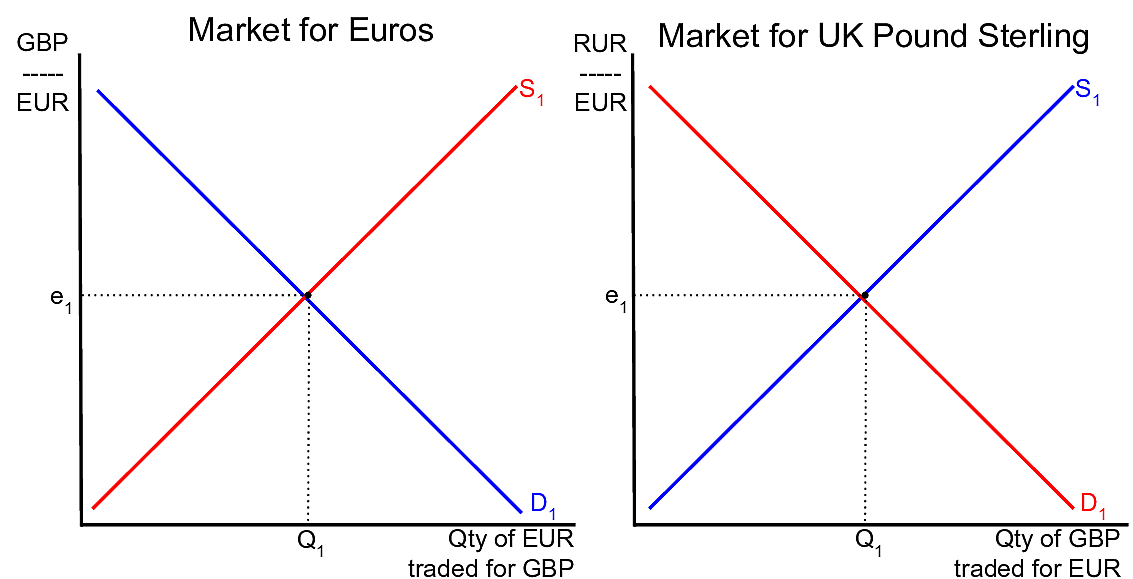
\includegraphics[width=0.8\linewidth]{./images/exchangerates-interestrates-EUR-GBP-start.jpg}}
    \only<2>{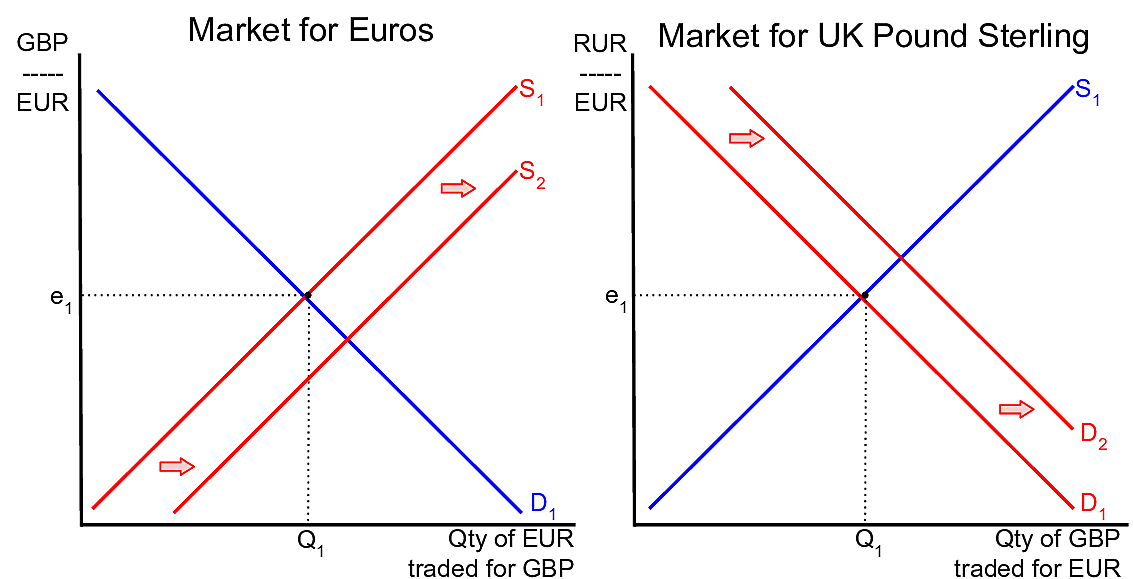
\includegraphics[width=0.8\linewidth]{./images/exchangerates-interestrates-EUR-GBP-oneshift.jpg}}
    \only<3->{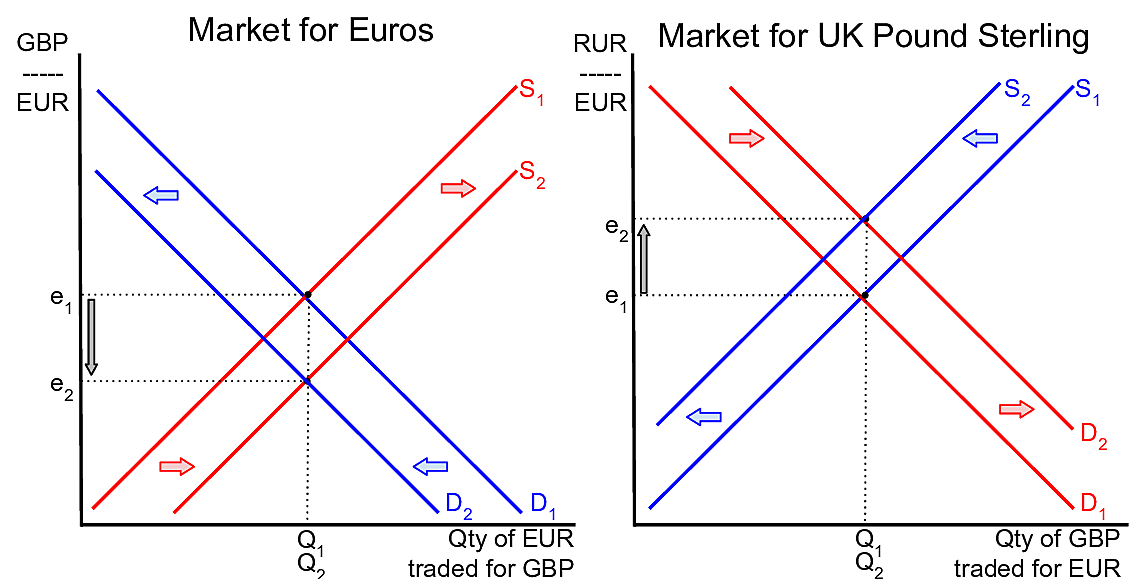
\includegraphics[width=0.8\linewidth]{./images/exchangerates-interestrates-EUR-GBP.jpg}}
  \end{center}
  \only<1>{Two related markets.  Market for Euro (Price=GBP/EUR)\newline and Market for U.K. Pound Sterling (Price=EUR/GBP)}
  \only<2>{Increase in Euro-area investors' demand for U.K. Pounds\newline$\rightarrow$ Increase in Supply of Euros}
  \only<3>{Decrease in British investor's demand for Euros\newline$\rightarrow$ Decrease in Supply of U.K. Pounds.}
  \only<4>{Euro depreciates against the U.K. Pound Sterling\newline$\rightarrow$ U.K. Pound Sterling appreciates against Euro}   \end{scriptsize}
}


\begin{frame}
  \frametitle{Scholar Spotlight: Dr. Mark\'eta Arltov\'a}

  \textbf{The Impact of Economic Sanctions on Russian Economy and RUB/USD Exchange Rate}, \textit{Journal of International Studies}, January 2018.

  \vspace*{-0.25pc}\begin{columns}
    \begin{small}
    \begin{column}{0.65\textwidth}
      \begin{block}{Economic Sanctions, Exchange Rates, and Food Prices}
        \begin{itemize}[leftmargin=0pc]
          \item International price of oil positively affects USD/RUB exchange rate
          \item International sanctions following Crimea annexation decreased USD/RUB 2014-2016
          \item Depreciation of RUB increased imported food prices
          \item Russia counteracted exchange rate impact with import restrictions, including on food
        \end{itemize}
      \end{block}
    \end{column}
    \end{small}

    \begin{column}{0.3\textwidth}
      
\includegraphics[width=\linewidth]{./images/arltova.jpg}

      \begin{footnotesize}
        \textbf{Dr. Mark\'eta Arltov\'a}\\
      \end{footnotesize}
      \begin{tiny}
        Associate Professor\\
        Department of Statistics and Probability\\
        University of Economics\\ Prague, Czech Republic\\
      \end{tiny}

    \end{column}
    \end{columns}
\end{frame}


\section{}
\subsection{Reading and Exercises}
\frame
{
  \ft{Reading and Exercises}
  \begin{itemize}
  \item<+-> Textbook: Module 47
  \item<+-> \textbf{Canvas Quiz due Wednesday 11:59 PM}.\newline Multiple-choice, 10 questions, unlimited attempts allowed, only best score counts
  \item<+-> \textbf{Homework/In-class Exercise due Friday 11:59 PM}. We will work together in class on Thursday.
  \end{itemize}
}




\end{document}
